This Chapter has introduced the idea of creating Variables within your program's code to store values. These variables can be stored in Global or Local Variables, and passed to Functions or Procedures using Parameters.

This Section will help you answer the following questions:
\begin{itemize}
  \item How do local and global variables work?
  \item What happens with Parameters when Functions and Procedures are called?
  \item How do Function's return a value?
  \item How does Pass by Reference work?
  \item How can I demonstrate or check the execution of a program with Variables?
\end{itemize}

\subsection{Variables} % (fold)
\label{sub:visualise_variables}

To get started let us have a look at the basic concept of Variables. Rather than working through the Simple Change Calculator program we can use a simpler program to start with. Understanding this will then help you understand what is happening in the Simple Change Calculator. The program we will use is in Listing \ref{plst:assignment-test}. This program will contain two variables that are local to the \texttt{main} function in C or the \texttt{Main} procedure in Pascal: \texttt{val} and \texttt{range}.

\pseudocode{plst:assignment-test}{Pseudocode illustrating variable use}{topics/storing-using-data/application/test-assignment.txt}


\subsubsection{Visualising Variables in the Computer} % (fold)
\label{ssub:visualising_variables_in_the_computer}

To get started understanding this let us return to the Conceptual Computer we have been using to explain how these concepts work.

\begin{itemize}
  \item Test Assignment's Program Launches, putting Main on the Stack.
  \item The assignment statement stores a value in the \texttt{val} Variable.
  \item The second assignment statements stores a value in the \texttt{range} Variable.
  \item The values of the Variables are output to the Terminal.
\end{itemize}

% subsubsection visualising_variables_in_the_computer (end)
\clearpage
\subsubsection{Test Assignment's Program Launches, putting Main on the Stack.} % (fold)
\label{ssub:test_assignment_s_program_launches_putting_main_on_the_stack_}

When the Program starts space is allocated on the Stack for the Program's Main Function or Procedure. When a Function or Procedure has \nameref{sub:local_variable}s, these are also allocated onto the Stack.

\begin{figure}[htbp]
   \centering
   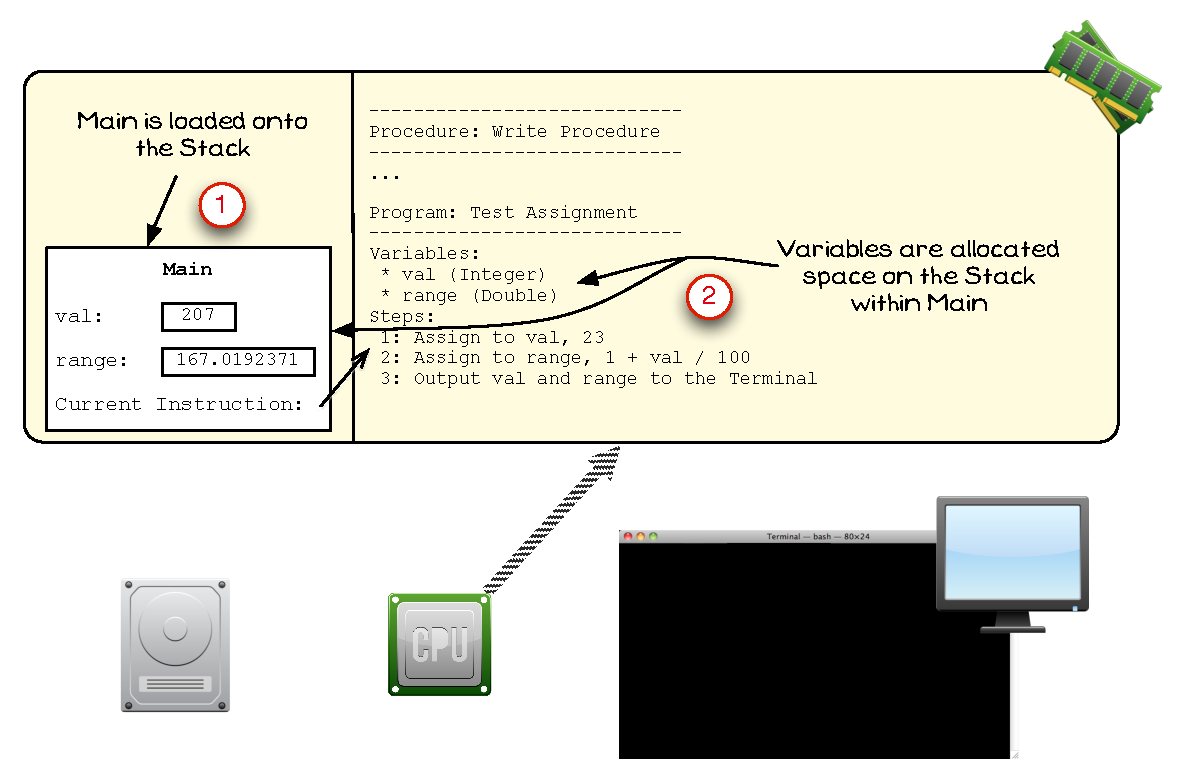
\includegraphics[width=\textwidth]{./topics/storing-using-data/images/vis-local-var-1} 
   \caption{Program's entry point is loaded onto the Stack}
   \label{fig:vis-data-local-1}
\end{figure}

\mynote{
\begin{itemize}
  \item The Program's instructions are loaded into memory when the program is executed.
  \item In Figure \ref{fig:vis-data-local-1} the indicated areas show the following:
  \begin{enumerate}
    \item When the Program starts, \texttt{Main} is loaded onto the Stack. This keeps track of all of the details related to the execution of \texttt{Main}.
    \item The Variables that are declared in \texttt{Main} are allocated space on the Stack.
  \end{enumerate}
  \item The two aspects of the Variable are shown in the illustration. The \textbf{variable} is the box drawn next to its name. The \textbf{value} is then written within the Variable.
  \item Notice that the variables each have a value to start with, even though the code has not yet assigned a value. The variable is allocated memory into which its value will be stored. \textbf{Memory is not automatically cleared} after its use, so the variables will get whatever value happened to be at that location previously.
  \item Each Variable is allocated enough space to stores its value. The \texttt{val} Variable needs 32 bits to store an \texttt{Integer} value, whereas the \texttt{range} Variable needs 64 bits to store its \texttt{Double} value.
\end{itemize}
}

% subsubsection test_assignment_s_program_launches_putting_main_on_the_stack_ (end)
\clearpage
\subsubsection{The assignment statement stores a value in the \texttt{val} Variable.} % (fold)
\label{ssub:the_assignment_statement_stores_a_value_in_the_val_variable_}

The first action of this program is to store the value 23 in the \texttt{val} Variable.

\begin{figure}[htbp]
   \centering
   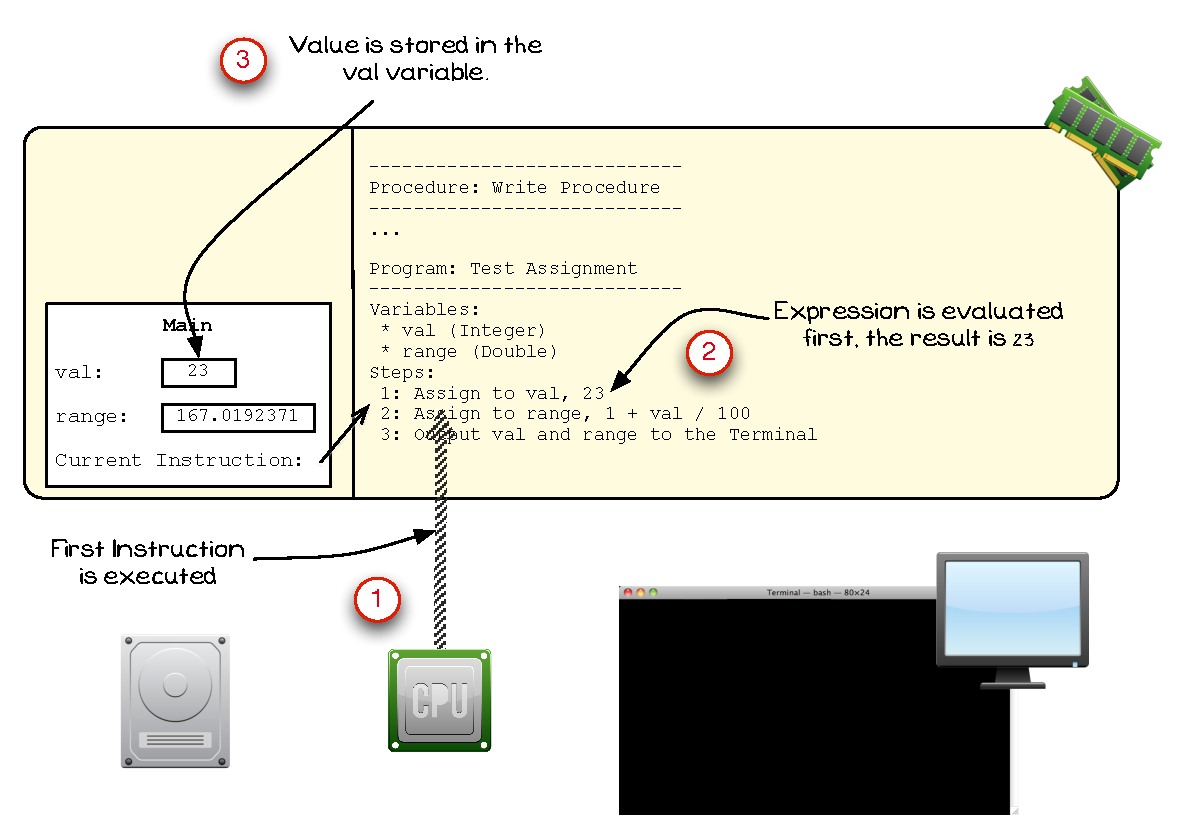
\includegraphics[width=\textwidth]{./topics/storing-using-data/images/vis-local-var-2} 
   \caption{The Assignment Statement assigns a value to the \texttt{val} Variable}
   \label{fig:vis-data-local-2}
\end{figure}

\mynote{
\begin{itemize}
  \item In Figure \ref{fig:vis-data-local-2} the indicated areas show the following:
  \begin{enumerate}
    \item The \nameref{sub:assignment_statement} is executed. This code has two sides. The right hand side executes first and needs to evaluate the Expression. Next the left hand side is used to determine where the resulting value needs to be stored.
    \item The value of the Expression is the Literal value 23.
    \item 23 is stored in the \texttt{val} Variable.
  \end{enumerate}
  \item Once this line of the Program has executed the \texttt{val} variable now has the value 23.
\end{itemize}
}

% subsubsection the_assignment_statement_stores_a_value_in_the_val_variable_ (end)

\clearpage
\subsubsection{The second assignment statements stores a value in the \texttt{range} Variable.} % (fold)
\label{ssub:the_second_assignment_statements_stores_a_value_in_the_range_variable_}

The next step in the program is to store the value \texttt{1 + val / 100} in the \texttt{range} Variable. This must read the value from the \texttt{val} Variable to determine the value to be stored.

\begin{figure}[htbp]
   \centering
   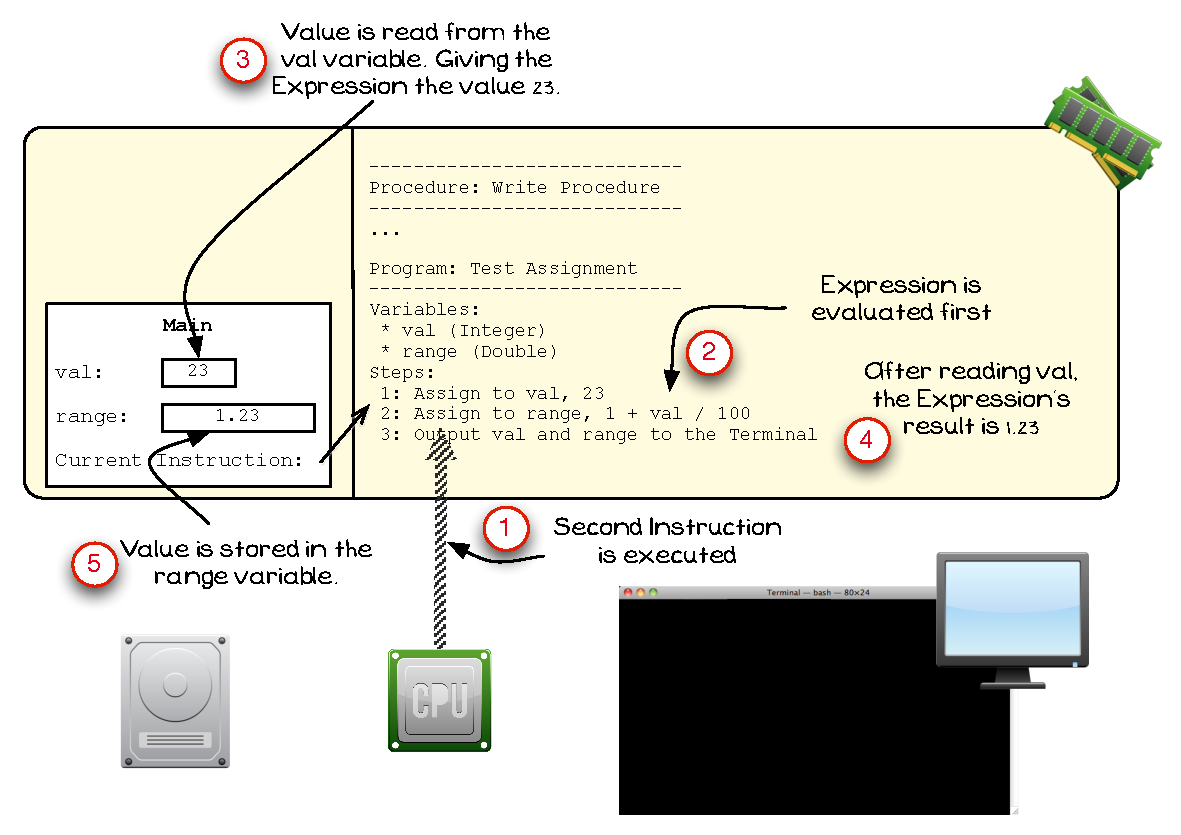
\includegraphics[width=\textwidth]{./topics/storing-using-data/images/vis-local-var-3} 
   \caption{The Assignment Statement assigns a value to the \texttt{val} Variable}
   \label{fig:vis-data-local-3}
\end{figure}

\mynote{
\begin{itemize}
  \item In Figure \ref{fig:vis-data-local-3} the indicated areas show the following:
  \begin{enumerate}
    \item The \nameref{sub:assignment_statement} is executed. As before, this needs to evaluate the Expression on the right hand side and store the result in the Variable on the left hand side.
    \item The first step to performing the assignment is to evaluate the expression. This requires the value from the \texttt{val} Variable.
    \item Within the Expression the value of \texttt{val} is read. At this point in the Program \texttt{val} has the value 23.
    \item The Expression is now \texttt{1 + 23 / 100}, giving the result \texttt{1.23}.
    \item The calculated value is then stored in the \texttt{range} Variable.
  \end{enumerate}
\end{itemize}
}

% subsubsection the_second_assignment_statements_stores_a_value_in_the_range_variable_ (end)

\clearpage
\subsubsection{The values of the Variables are output to the Terminal.} % (fold)
\label{ssub:the_values_of_the_variables_are_output_to_the_terminal_}

The third, and final, instruction in the Program's main function or procedure is to output the values of each of these variables to the Terminal. This uses the values from within the Variables to determine what is output.

\begin{figure}[htbp]
   \centering
   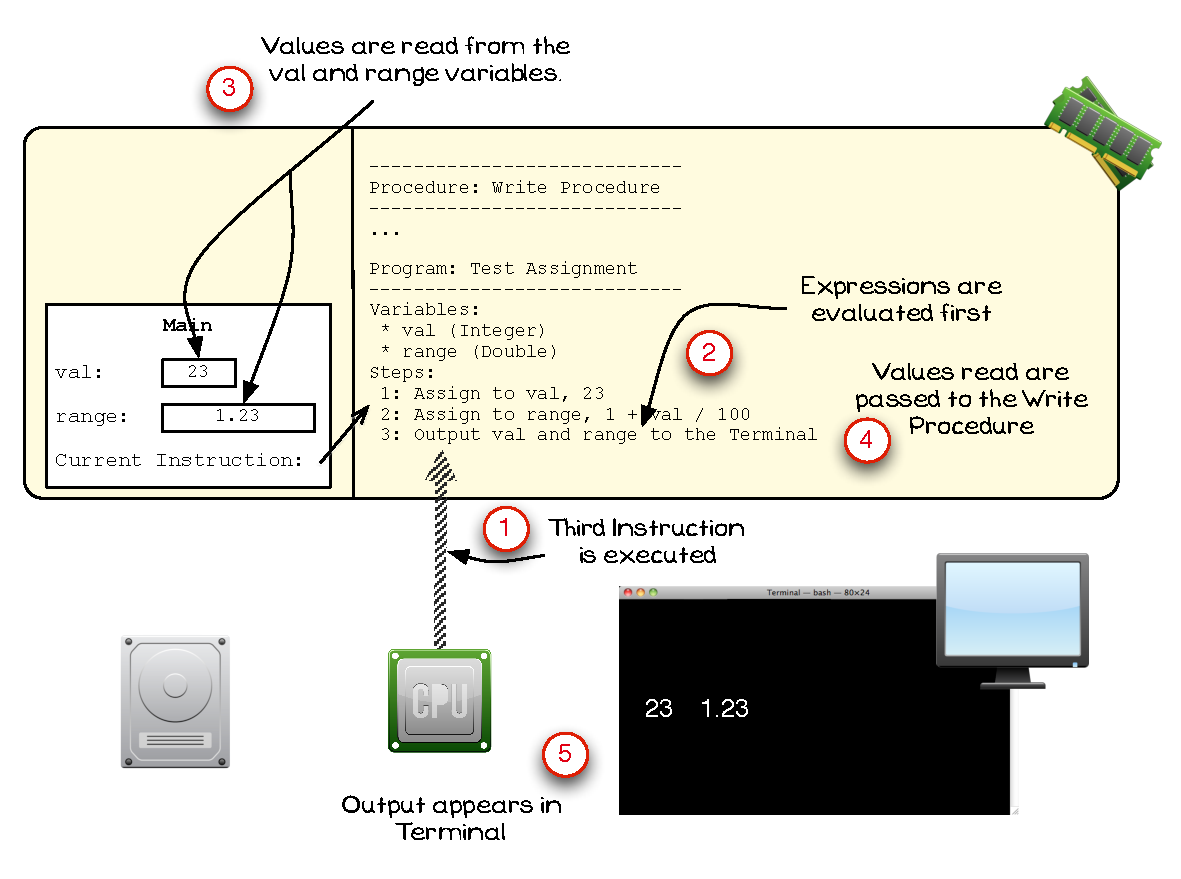
\includegraphics[width=\textwidth]{./topics/storing-using-data/images/vis-local-var-4} 
   \caption{The Assignment Statement assigns a value to the \texttt{val} Variable}
   \label{fig:vis-data-local-4}
\end{figure}

\mynote{
\begin{itemize}
  \item In Figure \ref{fig:vis-data-local-4} the indicated areas show the following:
  \begin{enumerate}
    \item The final instruction is a call to the output procedure of the language. This must be passed the data to output.
    \item The Write Procedure is passed a number of values to output.
    \item The values of the Variables will be read to get the argument values to pass.
    \item The values read from the Variables are then passed to the Write Procedure (\texttt{printf} in C, or \texttt{WriteLn} in Pascal).
    \item When the \texttt{Write Procedure} finishes its task the values will have been written to the Terminal.
  \end{enumerate}
\end{itemize}
}
% subsubsection the_values_of_the_variables_are_output_to_the_terminal_ (end)
% subsection local_variables (end)

\clearpage
\subsection{Parameters, Locals and Globals} % (fold)
\label{sub:visualise_parameters}

There are three locations at which you can declare variables. \emph{Global Variables} are declared within the program, \emph{Local Variables} are declared within Functions and Procedures, and \emph{Parameters} are used to pass values into Functions and Procedures.

\pseudocode{plst:test_proc_data}{Pseudocode used to examine how Global Variables, Local Variables, and Parameters work}{topics/storing-using-data/application/test-globals-and-locals.txt}

Listing \ref{plst:test_proc_data} is the code that we will use to demonstrate how these Variables work when code is executed by the Computer. This program does not have any meaningful purpose beyond interacting with Global Variables, Local Variables, and Parameters, so do not read too much into the actions being performed. What is important is to examine how the different variables work when the code is executed.

This Section will examine these Variables by looking at the following:
\begin{itemize}
  \item \nameref{ssub:memory_partitions_include_space_for_global_variables}
  \item \nameref{ssub:vars-program_is_loaded_into_memory}
  \item \nameref{ssub:initial_commands_occur}
  \item \nameref{ssub:passing_parameters_in_a_procedure_call}
  \item \nameref{ssub:test_params_commands_are_executed}
  \item \nameref{ssub:control_returns_to_main_when_test_params_ends}
\end{itemize}

\clearpage
\subsubsection{Memory Partitions include space for Global Variables} % (fold)
\label{ssub:memory_partitions_include_space_for_global_variables}

When the program is executed the Operating System allocates it space in memory. This space is partitioned into different areas, with each area storing an aspect of the program's data or instructions.

\begin{figure}[htbp]
   \centering
   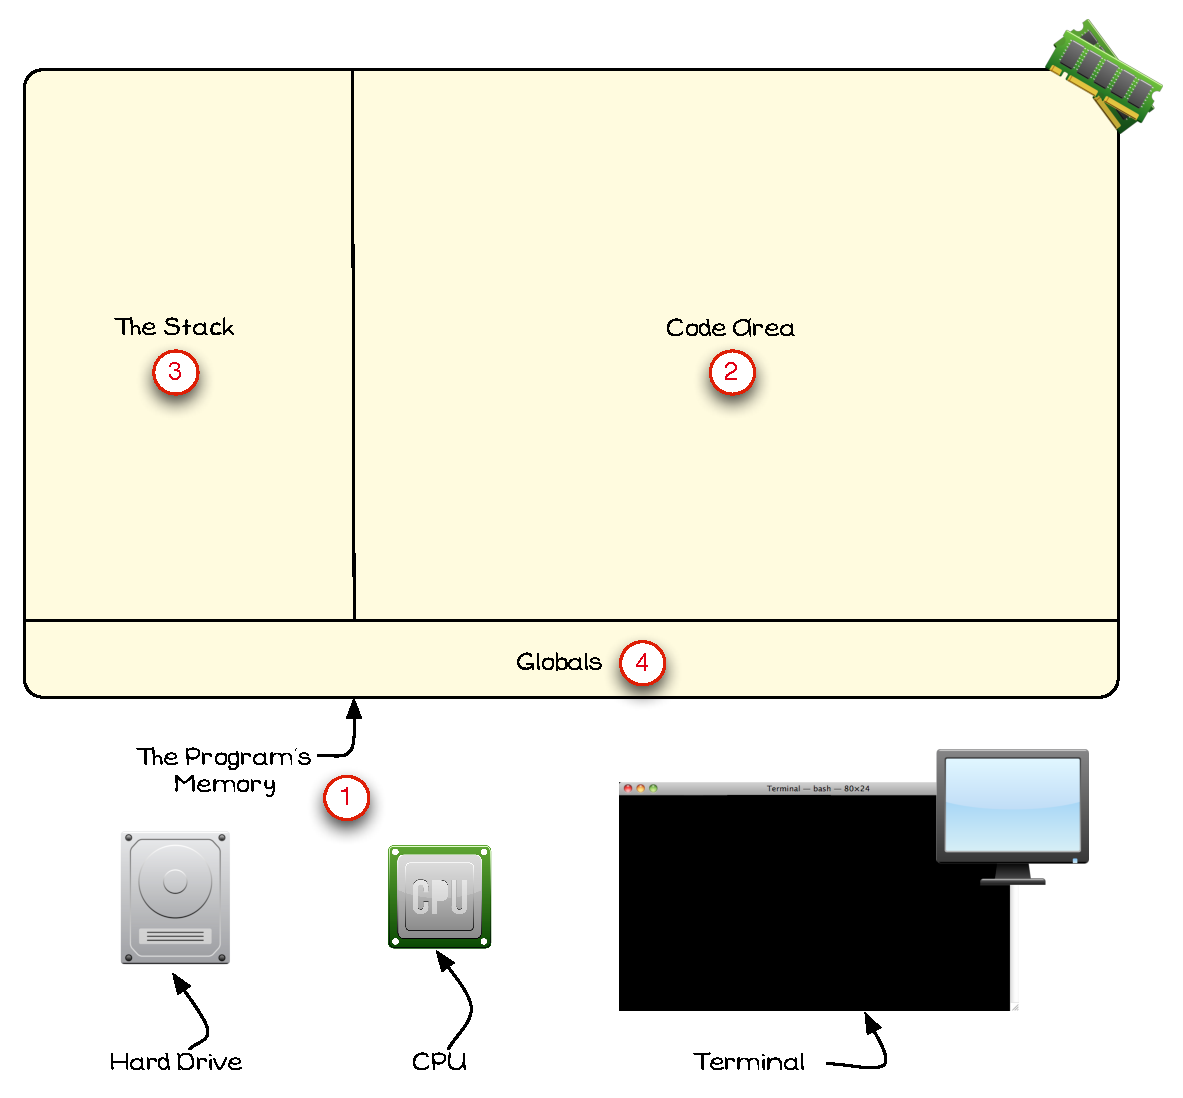
\includegraphics[width=0.9\textwidth]{./topics/storing-using-data/images/vis-globals-1} 
   \caption{Memory is partitioned into spaces for the Code, Stack, and Global Variables}
   \label{fig:vis-globals-1}
\end{figure}

\mynote{
\begin{itemize}
  \item In Figure \ref{fig:vis-globals-1} the indicated areas show the following:
  \begin{enumerate}
    \item The Program's memory is allocated by the Operation System, and divided into areas to store different kinds of values.
    \item The Program's instructions are loaded into the \textbf{Code Area}.
    \item The \textbf{Stack} is used to manage the execution of Functions and Procedures.
    \item \textbf{Global} Variables are stored in their own area of memory.
  \end{enumerate}
\end{itemize}
}

% subsubsection memory_partitions_include_space_for_global_variables (end)

\clearpage

\subsubsection{Program is loaded into memory} % (fold)
\label{ssub:vars-program_is_loaded_into_memory}

When the program is executed its global variables are allocated space, and then the main code is executed.

\begin{figure}[htbp]
   \centering
   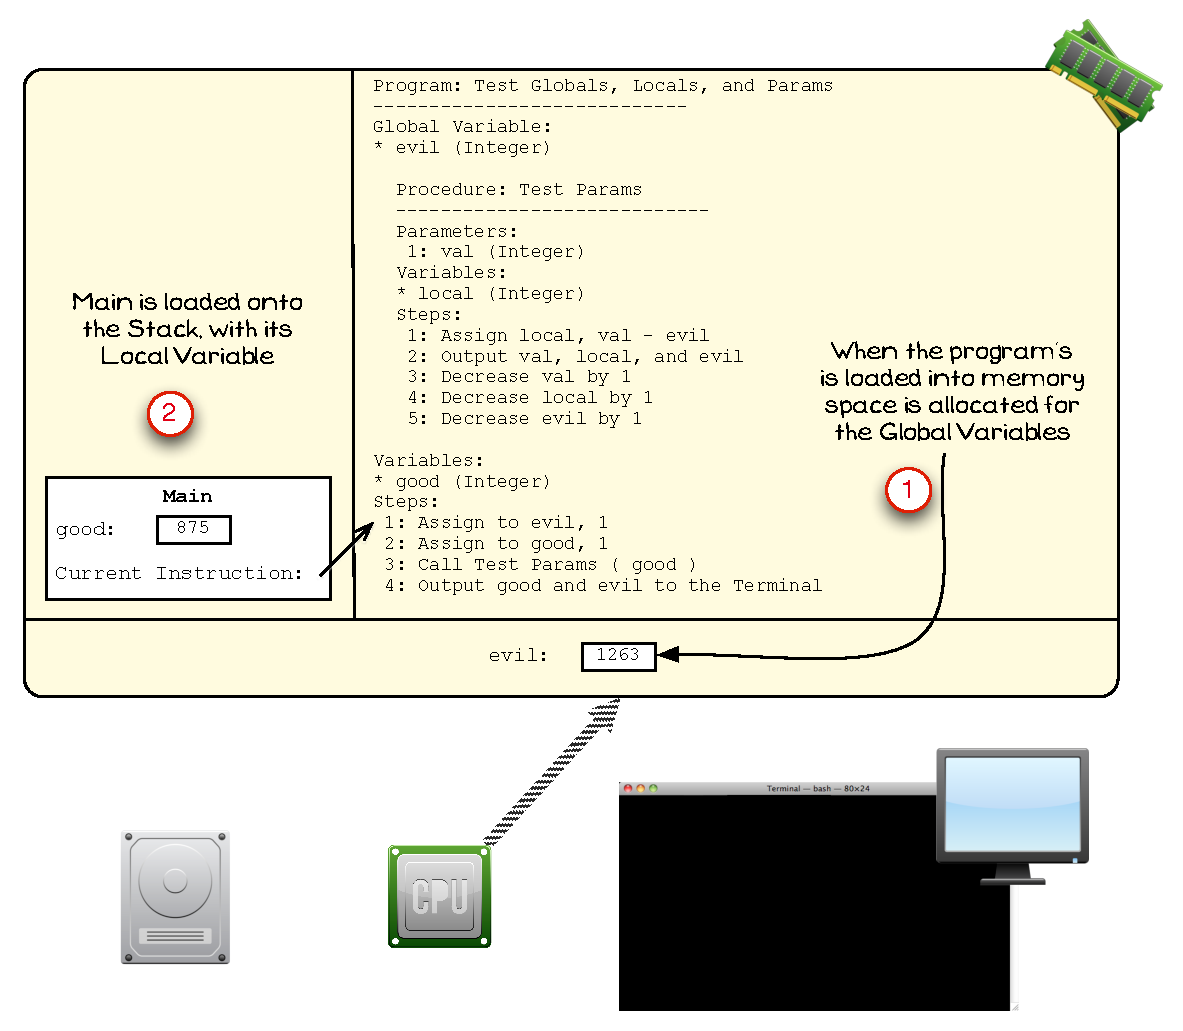
\includegraphics[width=\textwidth]{./topics/storing-using-data/images/vis-globals-2} 
   \caption{The Global Variables are allocated space, then the Entry Point is loaded onto the Stack}
   \label{fig:vis-globals-2}
\end{figure}

\mynote{
\begin{itemize}
  \item In Figure \ref{fig:vis-globals-2} the indicated areas show the following:
  \begin{enumerate}
    \item The global variables are allocated space when the program is loaded. Some Operating Systems ensure that this memory is cleared by zeroing each value, but others do not so you cannot rely upon the value these variables will have when they are loaded unless you initialise it yourself with an Assignment Statement.
    \item The main code is then loaded onto the Stack, with space for its local variable.
  \end{enumerate}
\end{itemize}
}

% subsection program_is_loaded_into_memory (end)
\clearpage

\subsubsection{Initial Commands Occur} % (fold)
\label{ssub:initial_commands_occur}

The program executes each of the statements, one at a time. Figure \ref{fig:vis-globals-3} shows the values in memory by the time the Computer has completed the execution of the first two commands.

\begin{figure}[htbp]
   \centering
   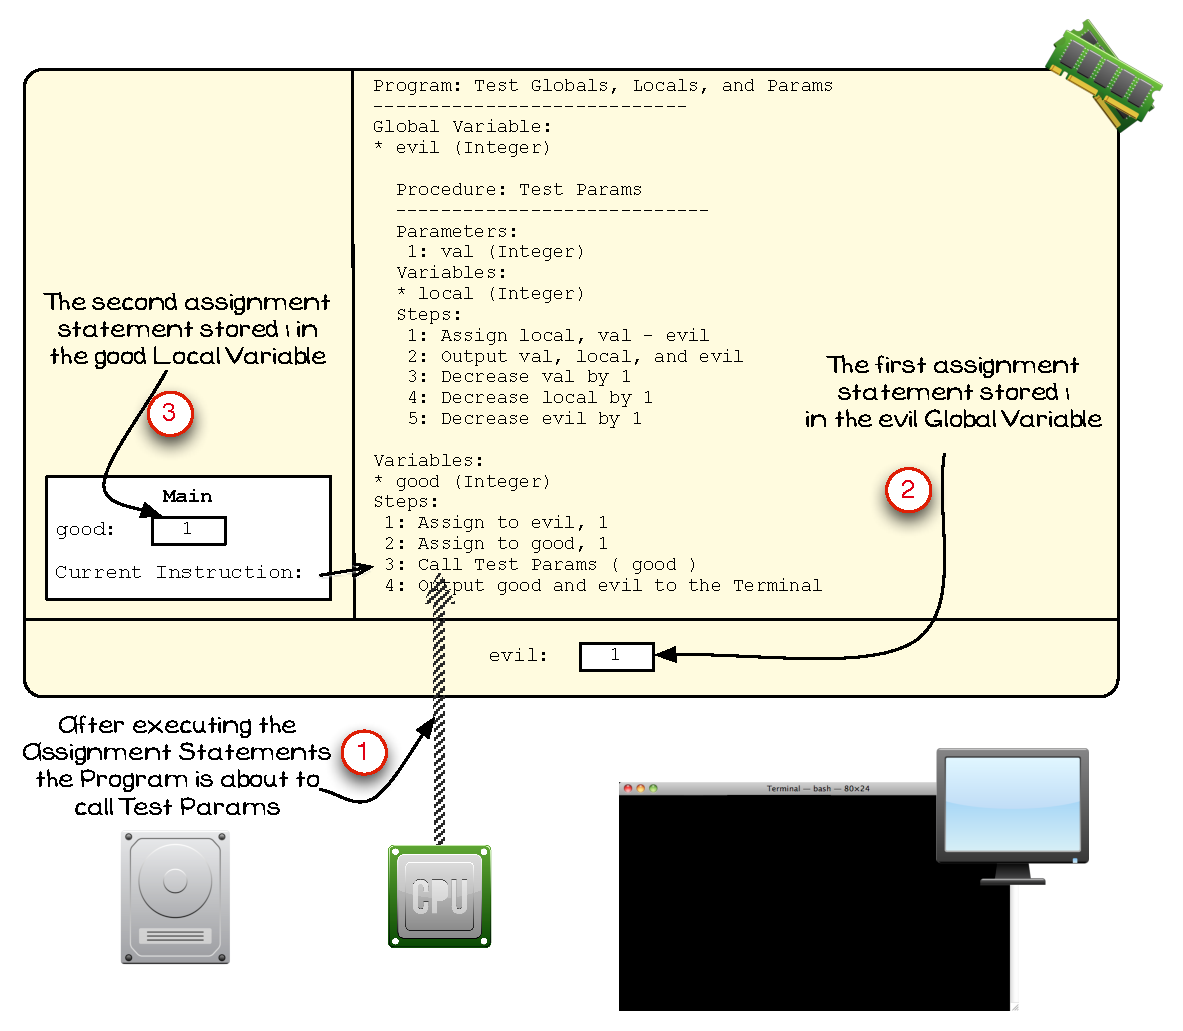
\includegraphics[width=\textwidth]{./topics/storing-using-data/images/vis-globals-3} 
   \caption{The instructions store values in the different variables}
   \label{fig:vis-globals-3}
\end{figure}

\mynote{
\begin{itemize}
  \item In Figure \ref{fig:vis-globals-3} the indicated areas show the following:
  \begin{enumerate}
    \item This picture is showing the computer at the point just before it executes the call to \texttt{Test Params}.
    \item The first assignment statement assigned the value \texttt{1} to the \texttt{evil} Global Variable.
    \item The second assignment statement assigned the value \texttt{1} to the \texttt{good} Local Variable.
  \end{enumerate}
\end{itemize}
}

% subsubsection initial_commands_occur (end)

\clearpage

\subsubsection{Passing Parameters in a Procedure Call} % (fold)
\label{ssub:passing_parameters_in_a_procedure_call}

At this point the Computer is executing the call to \texttt{Test Params}. This involves passing a value to the \texttt{val} parameter.

\begin{figure}[htbp]
   \centering
   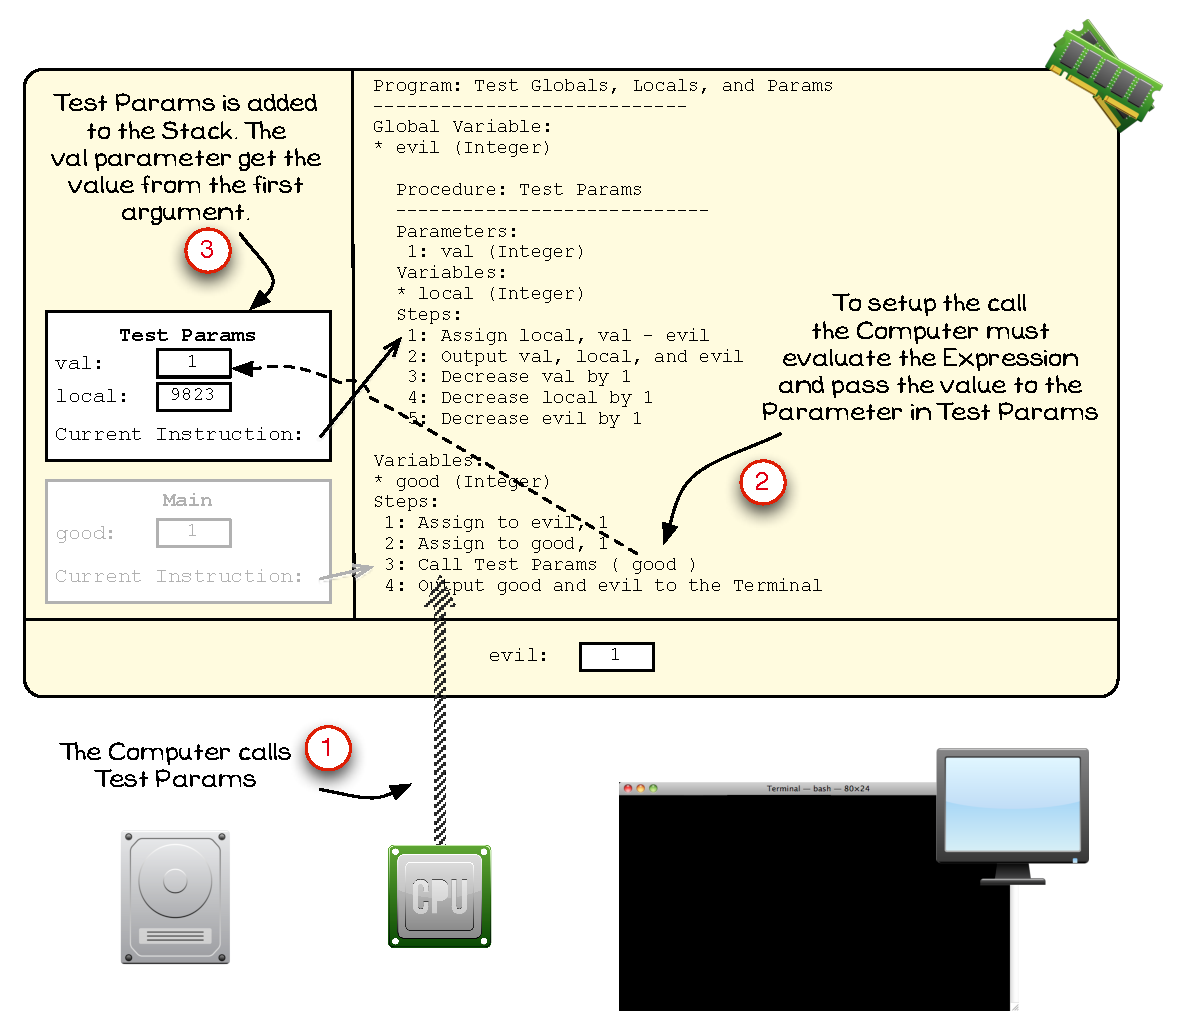
\includegraphics[width=\textwidth]{./topics/storing-using-data/images/vis-globals-4} 
   \caption{The \emph{value} of the Argument is passed to the Parameter when the Procedure is called}
   \label{fig:vis-globals-4}
\end{figure}

\mynote{
\begin{itemize}
  \item In Figure \ref{fig:vis-globals-4} the indicated areas show the following:
  \begin{enumerate}
    \item The Computer calls the \texttt{Test Params} procedure. This must be passed a single value that will be copied into the \texttt{val} Parameter.
    \item The first part of the call requires the Computer to evaluate the Expression being passed to the Procedure. In this case that involves reading the \texttt{good} Local Variable and passing its \emph{value} to the Parameter.
    \item Once the values for the Parameters are determined, the next step is to allocate space for \texttt{Test Params} on the Stack. Within \texttt{Test Params} there will be space allocated for the \texttt{val} parameter, as well as space allocated for the \texttt{local} Local Variable. The value of the \emph{argument} is copied into the \emph{parameter}, and the called Function or Procedure's code can now execute. In this case the value \texttt{1} is stored in \texttt{val}.
  \end{enumerate}
\end{itemize}
}


% subsubsection passing_parameters_in_a_procedure_call (end)
\clearpage

\subsubsection{Test Params Commands are Executed} % (fold)
\label{ssub:test_params_commands_are_executed}

The commands in \texttt{Test Params} are executed one at a time. These instructions will interact with the Variables that are visible to the \texttt{Test Params} Procedure, which include its Local Variables as well as the Global Variables.

\begin{figure}[htbp]
   \centering
   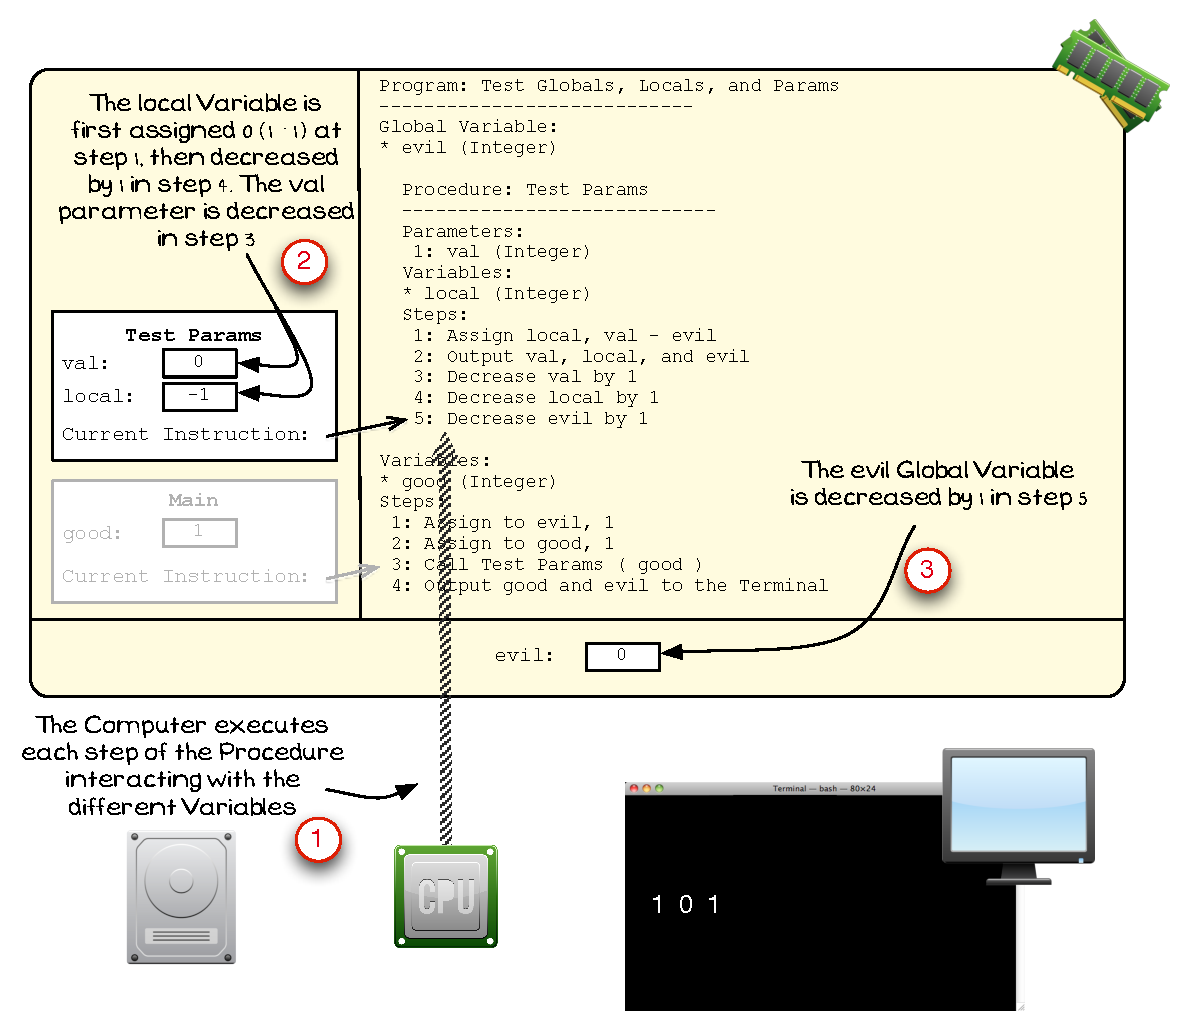
\includegraphics[width=\textwidth]{./topics/storing-using-data/images/vis-globals-5} 
   \caption{Steps in \texttt{Test Params} execute, altering values in the Variables}
   \label{fig:vis-globals-5}
\end{figure}

\mynote{
\begin{itemize}
  \item In Figure \ref{fig:vis-globals-5} the indicated areas show the following:
  \begin{enumerate}
    \item Each instruction is executed one at a time. This picture shows the instructions at the end of the last instruction in \texttt{Test Params} before it ends.
    \item The steps of the Procedure are able to read and write values to the Function or Procedure's Parameters and Local Variables, as shown here.
    \item The Procedure is also able to read and write values to the Global Variables.
  \end{enumerate}
  \item Notice that \texttt{Test Params} cannot see the \texttt{good} Variable. It exists within the \texttt{Main} code and cannot be accessed from other Functions or Procedures.
  \item You can decrease the value of a Variable using an Assignment Statement. For example `\texttt{Assign to val, the value val - 1}'. This will read the current value from the \texttt{val} Variable, subtract one from that, and then store the result back in the \texttt{val} variable.
\end{itemize}
}
% subsubsection test_params_commands_are_executed (end)

\clearpage

\subsubsection{Control returns to Main when Test Params ends} % (fold)
\label{ssub:control_returns_to_main_when_test_params_ends}

When \texttt{Test Params} ends control returns to the Program's main code. The space allocated to \texttt{Test Params} is now released, including the space allocated to the \texttt{val} Parameter and the \texttt{local} Variable.

\begin{figure}[htbp]
   \centering
   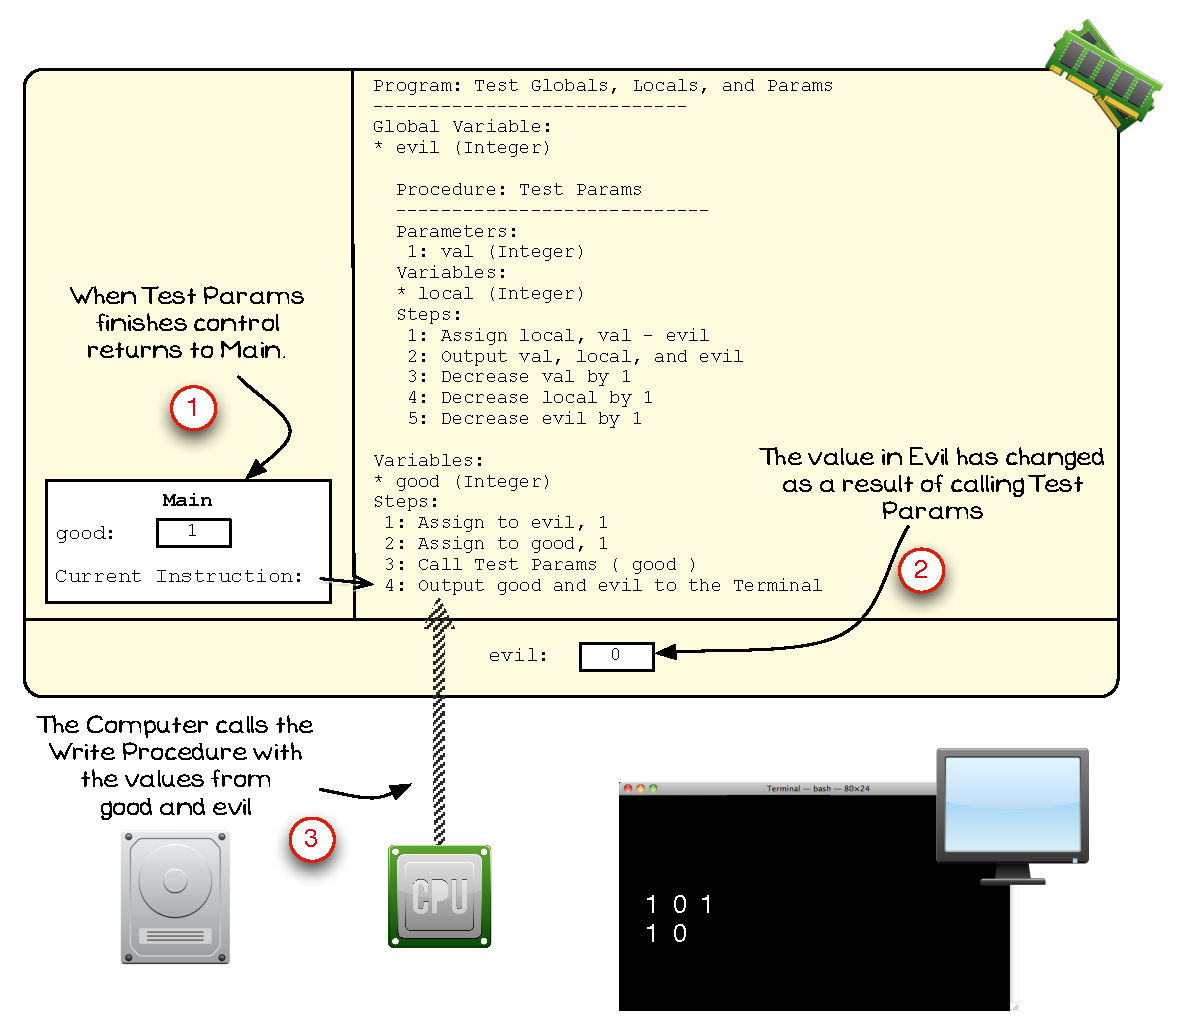
\includegraphics[width=\textwidth]{./topics/storing-using-data/images/vis-globals-6} 
   \caption{Control returns to Main when \texttt{Test Params} ends}
   \label{fig:vis-globals-6}
\end{figure}

\mynote{
\begin{itemize}
  \item In Figure \ref{fig:vis-globals-6} the indicated areas show the following:
  \begin{enumerate}
    \item Control returns to \texttt{Main} when \texttt{Test Params} ends.
    \item Notice that the value of the \texttt{evil} Global Variable has changed as a side effect of running \texttt{Test Params}. This is easy to follow in a small program, but can cause difficulties when you start building larger programs. As a result, Global Variables should be avoided.
    \item The last instruction in the main code outputs the values of \texttt{good} and \texttt{evil} to the Terminal.
  \end{enumerate}
  \item The value within \texttt{good} has been passed to the \texttt{val} Parameter in \texttt{Test Params}. This copies the \emph{value}, not the \texttt{Variable}, as it is using the standard \emph{Pass by Value} mechanism. This means the code in \texttt{Test Params} has no way of affecting the value in the \texttt{good} Variable.
\end{itemize}
}

% subsection control_returns_to_main_when_test_params_ends (end)
\clearpage

% subsection parameters (end)

\subsection{Function Return Values} % (fold)
\label{sub:visualise_function_return_values}

The next kind of data is the result returned by a call to a Function. A Function is just like a Procedure, except that it calculates a value and is therefore called from within an Expression. To examine how this works within the Computer we will see how the code in Listing \ref{plst:function-test} executes. This code declares a \texttt{Square} function that calculates the square of a number (\texttt{val} passed in as a Parameter).   

\pseudocode{plst:function-test}{Function example, to illustrate how data is returned from a Function}{topics/storing-using-data/application/test-function.txt}

This Section will examine how Functions return values by looking at the following:
\begin{itemize}
  \item \nameref{ssub:test_functions_is_loaded_into_memory}
  \item \nameref{ssub:square_function_is_called}
  \item \nameref{ssub:square_s_result_is_calculated}
  \item \nameref{ssub:returned_value_is_used}
\end{itemize}

\clearpage
\subsubsection{Test Functions is loaded into memory} % (fold)
\label{ssub:test_functions_is_loaded_into_memory}

When the program is executes the Operating System loads its code into memory, and starts the main code running on the Stack.

\begin{figure}[htbp]
   \centering
   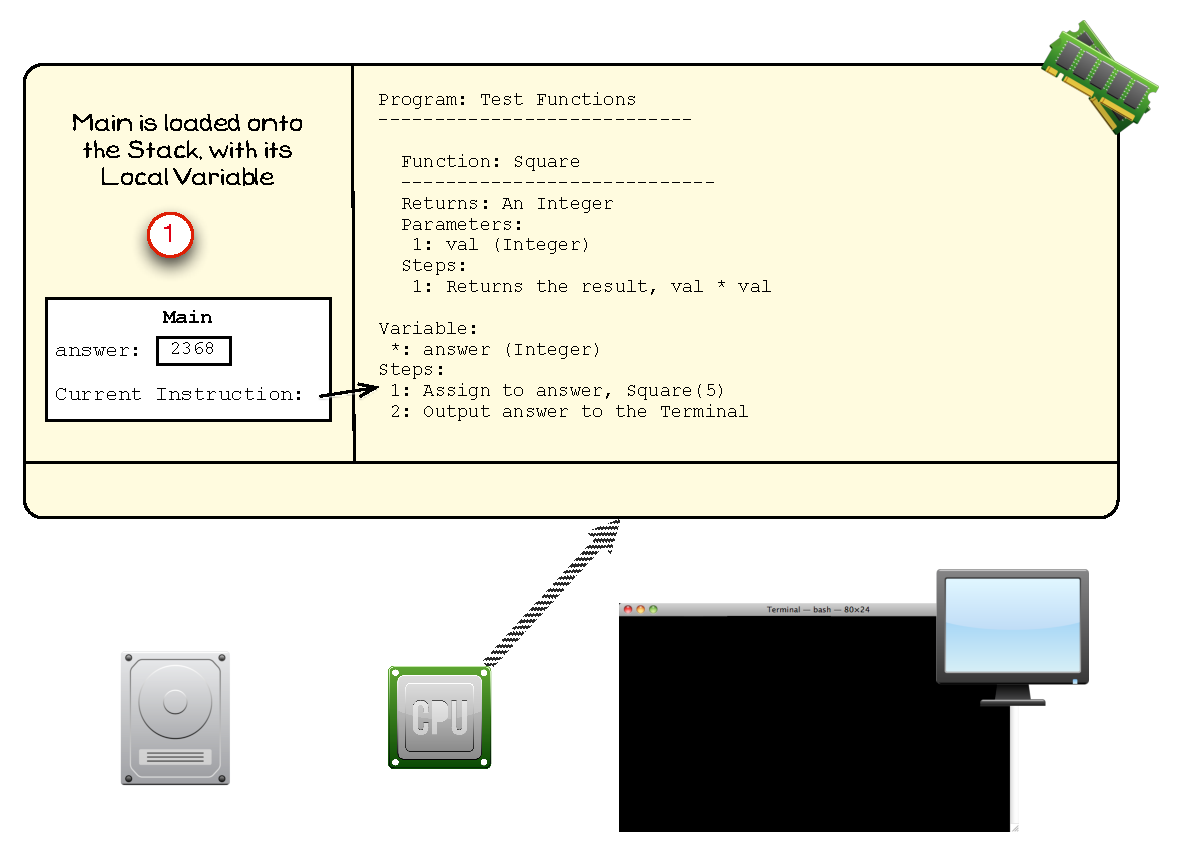
\includegraphics[width=\textwidth]{./topics/storing-using-data/images/vis-func-1} 
   \caption{Code is loaded into Memory and Main is loaded onto the Stack}
   \label{fig:vis-func-1}
\end{figure}

\mynote{
\begin{itemize}
  \item In Figure \ref{fig:vis-func-1} the indicated areas show the following:
  \begin{enumerate}
    \item Main is loaded onto the Stack, with space for its \texttt{answer} local variable.
  \end{enumerate}
  \item Notice the Global Variables section is empty as this program does not use Global Variables.
\end{itemize}
}

% subsubsection test_functions_is_loaded_into_memory (end)

\clearpage

\subsubsection{Square Function is Called} % (fold)
\label{ssub:square_function_is_called}

The \texttt{Square} function is called in the same way that a Procedure would be called. It is given space on the Stack, and its instructions are run.

\begin{figure}[htbp]
   \centering
   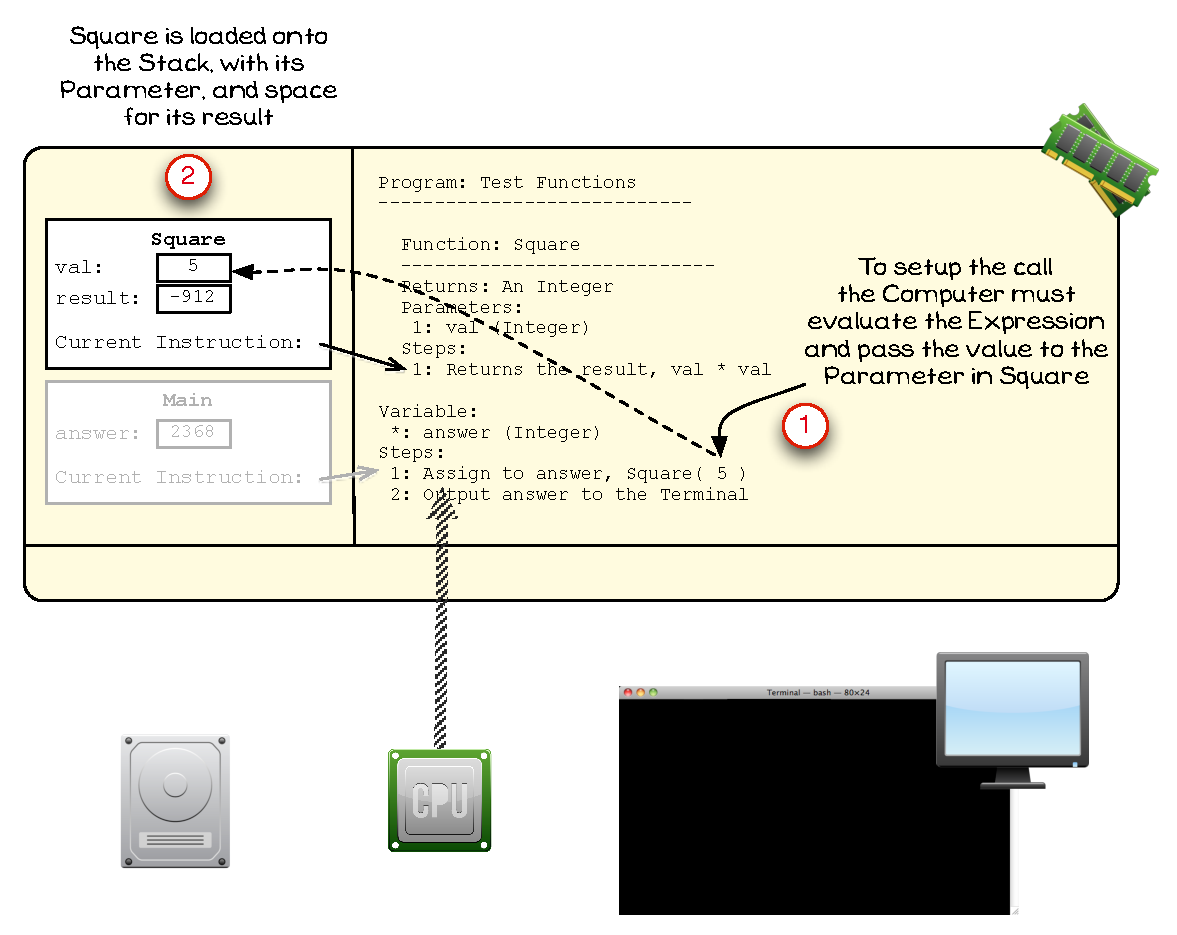
\includegraphics[width=\textwidth]{./topics/storing-using-data/images/vis-func-2} 
   \caption{\texttt{Square} is called, with the value 5 passed to its \texttt{val} Parameter}
   \label{fig:vis-func-2}
\end{figure}

\mynote{
\begin{itemize}
  \item In Figure \ref{fig:vis-func-2} the indicated areas show the following:
  \begin{enumerate}
    \item When the main code calls \texttt{Square} it passed in the value \texttt{5}, calculated simply by reading the Literal value.
    \item \texttt{Square} is added to the top of the Stack, and its \texttt{val} parameter is assigned the value passed in from the Function Call. In addition to any Parameter and Local Variables the Function also has space for its \texttt{result}. This will be the value returned to the caller when the Function ends.
  \end{enumerate}
  \item The value of the result will initially be whatever happens to be at that location in memory the last time it was used. You must make sure you assign a value to this within the Function.
\end{itemize}
}

\csection{In C the \nameref{sub:return_statement} assigns the value returned by the Function. There is no special \texttt{result} Variable that you can interact with. Conceptually, however, the value must be stored in order to be returned by the Function. In C the compiler takes care of these details for you.}



% subsubsection square_function_is_called (end)

\clearpage

\subsubsection{Square's result is calculated} % (fold)
\label{ssub:square_s_result_is_calculated}

Within the \texttt{Square} function its result is calculated and returned.

\begin{figure}[htbp]
   \centering
   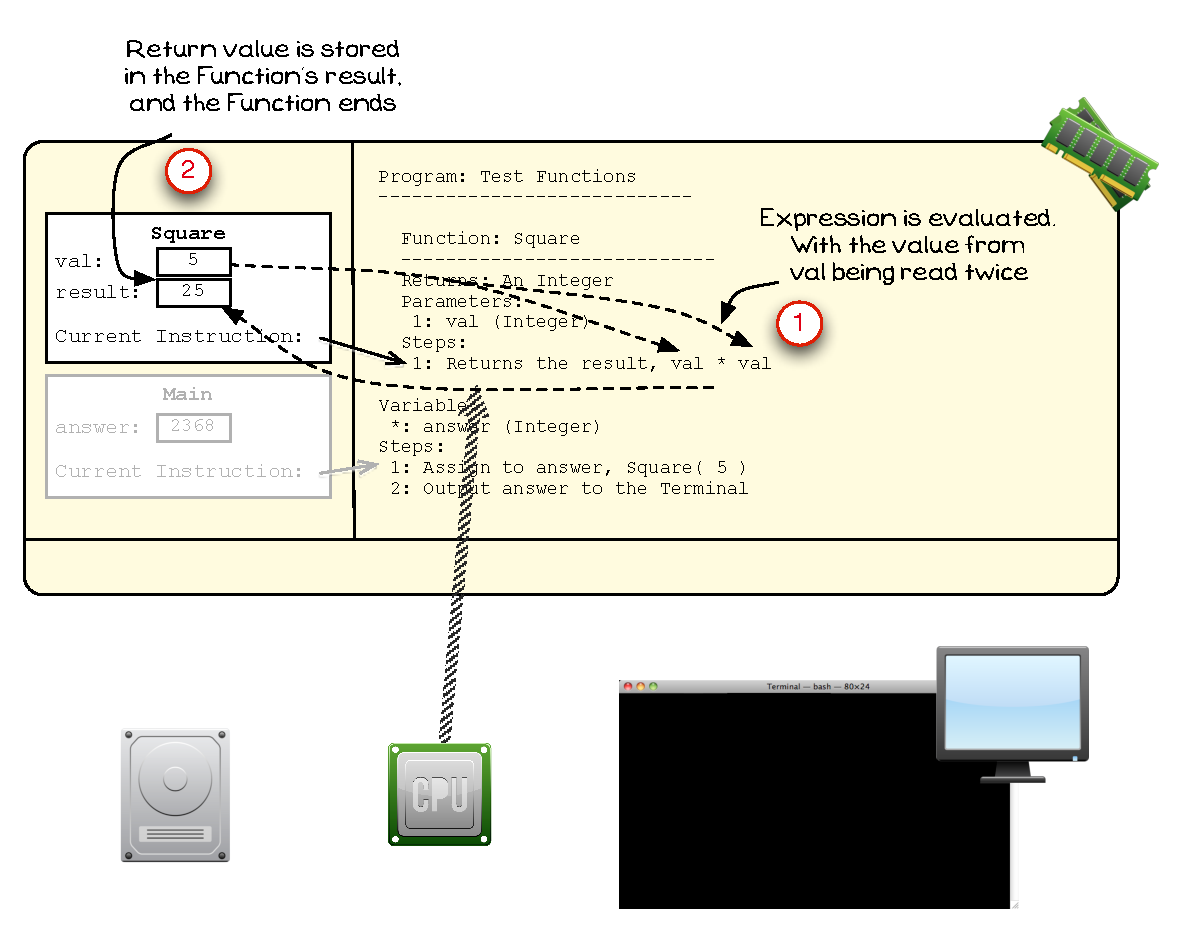
\includegraphics[width=\textwidth]{./topics/storing-using-data/images/vis-func-3} 
   \caption{\texttt{Square} prepares the value that will be returned to the caller}
   \label{fig:vis-func-3}
\end{figure}

\mynote{
\begin{itemize}
  \item In Figure \ref{fig:vis-func-3} the indicated areas show the following:
  \begin{enumerate}
    \item The expression `\texttt{val * val}' is evaluated. This reads the value of the \texttt{val} variable twice and multiplies the two values read. In this case this will calculate `\texttt{5 * 5}', giving \texttt{25}.
    \item The result of the expression is returned, setting the Function's result.
  \end{enumerate}
\end{itemize}
}

\csection{In C this is accomplished with the \nameref{sub:return_statement}. It assigns the result for the function and ends the Function at the same time.}

\passection{In Pascal you directly store the value in the special \texttt{result} Variable. This will not end the Function directly, but does store the value to be returned by the Function.}


% subsubsection square_s_result_is_calculated (end)
\clearpage

\subsubsection{Returned value is used} % (fold)
\label{ssub:returned_value_is_used}

When the Function ends, control is returned to the main code. This called the Function in order to evaluate an Expression. That expression will now continue to be evaluated using the value returned by the Function.

\begin{figure}[htbp]
   \centering
   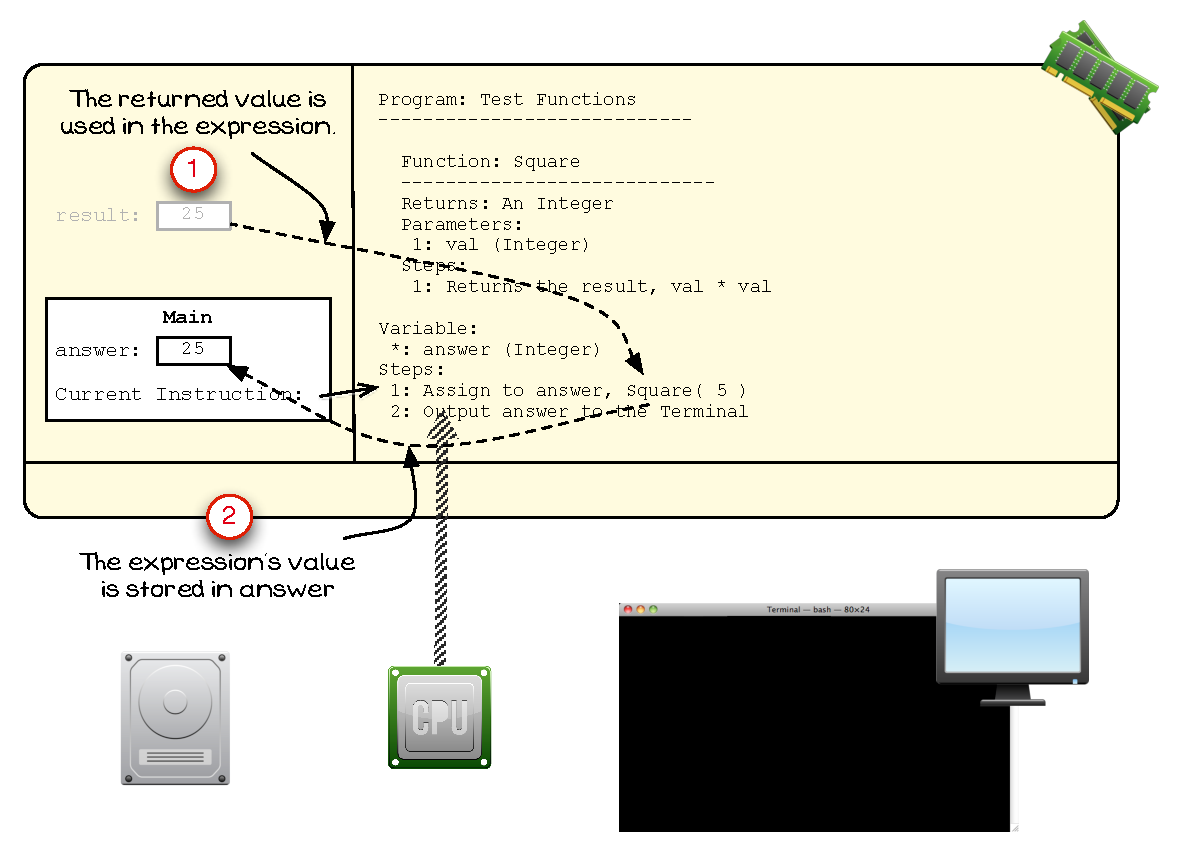
\includegraphics[width=\textwidth]{./topics/storing-using-data/images/vis-func-4} 
   \caption{The result of calling \texttt{Square} is used within the Expression, and the value is stored in \texttt{answer}}
   \label{fig:vis-func-4}
\end{figure}

\mynote{
\begin{itemize}
  \item In Figure \ref{fig:vis-func-4} the indicated areas show the following:
  \begin{enumerate}
    \item The result of the Function is made available to the caller. This will be read as part of the Function Call, and is then used within the Expression.
    \item In this case the Expression does not alter the value returned by the Function, and the result is stored in the \texttt{answer} variable.
  \end{enumerate}
  \item The expression that contains the Function Call can operate on the result returned from the function in the same way that it uses any other value. For example, the following expression is valid: \texttt{3 + Square(-7) * 5 + Square(Square(2))}.
  \item The key is to think of each Function Call as a value. So nested Function Calls like \texttt{Square(Square(2))} can be broken down into their individual values. In this example \texttt{Square(2)} is evaluated first, and returns the value \texttt{4}. This is then passed to the outer Function Call giving \texttt{Square(4)} and a final result of \texttt{16}.
\end{itemize}
}

% subsubsection returned_value_is_used (end)
% subsection function_return_values (end)

\clearpage
\subsection{Pass by Reference} % (fold)
\label{sub:visualise_pass_by_reference}

Working with data involves working with Variables of one form or another. When thinking about Variables it is important to realise the two aspects of each Variable: the \emph{Variable} and its \emph{value}. The \emph{Variable} is a location in memory, it is a place at which you can store a value. The \emph{value} within the Variable is a separate concern. This value can be read from the Variable in Expressions.

\pseudocode{plst:pass-by-ref-test}{Example used to illustrate how Pass by Reference works with the standard input Functions and Procedures.}{topics/storing-using-data/application/test-input.txt}

This Section will examine how Pass by Reference works by looking at the following:
\begin{itemize}
  \item \nameref{ssub:main_starts_and_a_prompt_is_written_for_the_user}
  \item \nameref{ssub:the_input_procedure_is_called_to_read_a_value_into_age}
  \item \nameref{ssub:the_input_procedure_stores_the_value_read_from_the_user_into_}
  \item \nameref{ssub:control_returns_to_main_and_}
\end{itemize}

\csection{In C the \texttt{Read Input Procedure} is the \texttt{scanf()} Function. This requires that you pass in a format string that indicates what will be read as well as passing in the Variables into which these values will be stored. You can read about this in \nameref{sub:c_terminal_input}. Step 2 from Listing \ref{plst:pass-by-ref-test} can be implemented in C using \csnipet{scanf("\%d", \&age);}.}

\clearpage
\subsubsection{Main starts and a prompt is written for the user} % (fold)
\label{ssub:main_starts_and_a_prompt_is_written_for_the_user}

The Program starts as normal with the Operating System allocating space for the Stack, Code, and Global Variables. Main is then loaded onto the Stack and its instructions are executed.

\begin{figure}[htbp]
   \centering
   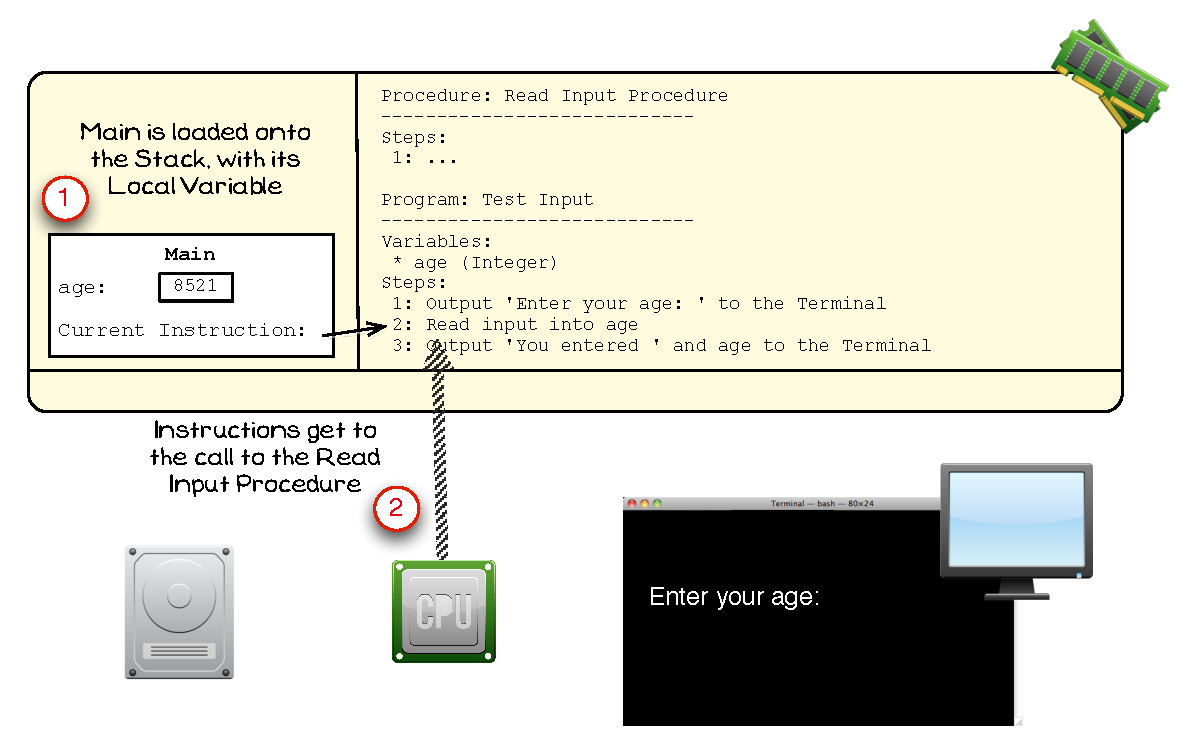
\includegraphics[width=\textwidth]{./topics/storing-using-data/images/vis-ref-1} 
   \caption{Code is loaded into Memory, Main is started, and the first instruction outputs a prompt}
   \label{fig:vis-ref-1}
\end{figure}

\mynote{
\begin{itemize}
  \item In Figure \ref{fig:vis-ref-1} the indicated areas show the following:
  \begin{enumerate}
    \item Main is loaded onto the stack, with space for the \texttt{age} Variable.
    \item The first instruction outputs `Enter your age: ' to the Terminal.
  \end{enumerate}
  \item When writing a prompt it is a good idea to keep the output on a single line. Just write the prompt without writing a new line.
\end{itemize}
}

% subsubsection main_starts_and_a_prompt_is_written_for_the_user (end)

\clearpage
\subsubsection{The Input Procedure is called to read a value into \texttt{age}} % (fold)
\label{ssub:the_input_procedure_is_called_to_read_a_value_into_age}

The next instruction in the main code is to call the Language's input procedure to read a value from the user and to store that value in the \texttt{age} variable. In order to achieve this you must pass the \texttt{age} variable itself to this procedure. That will enable the input code to store the value it reads into the variable that you give it.

\begin{figure}[htbp]
   \centering
   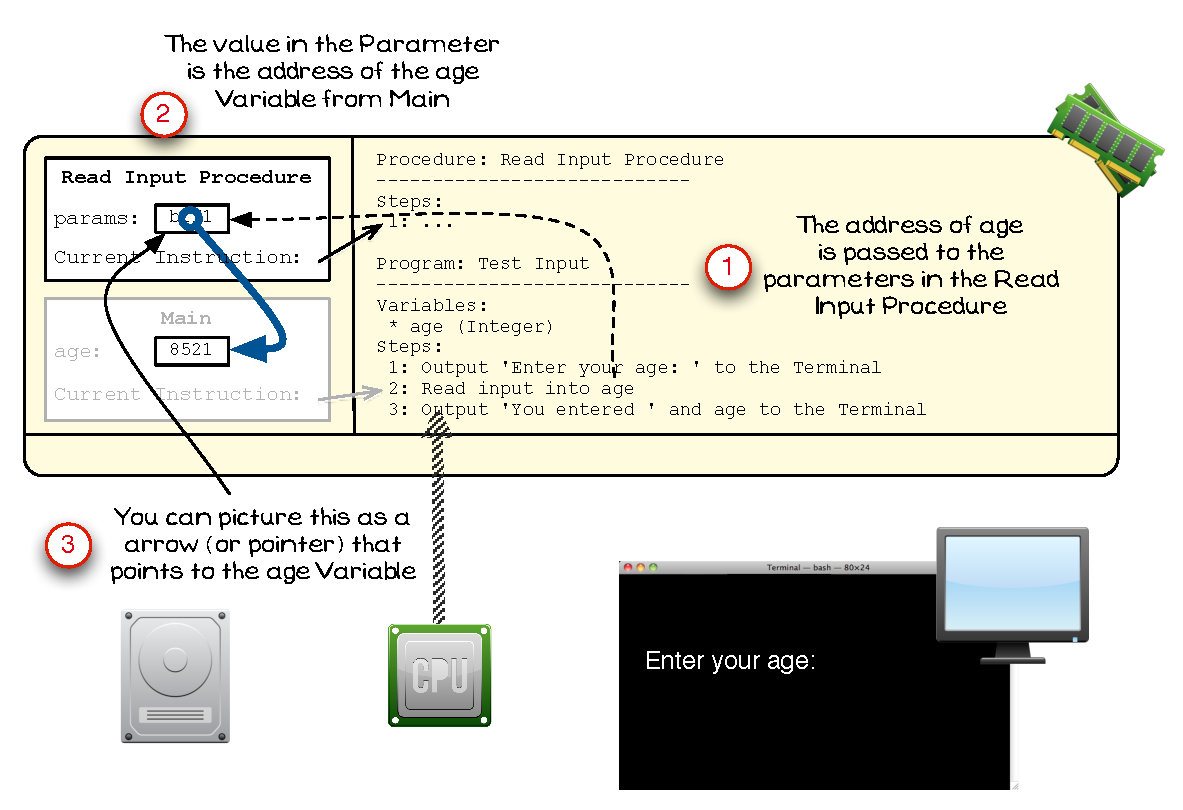
\includegraphics[width=\textwidth]{./topics/storing-using-data/images/vis-ref-2} 
   \caption{The input procedure starts, and the age Variable is passed to the Parameters}
   \label{fig:vis-ref-2}
\end{figure}

\mynote{
\begin{itemize}
  \item In Figure \ref{fig:vis-ref-2} the indicated areas show the following:
  \begin{enumerate}
    \item A variable is a location in memory, so it is not possible to actually move this location into the Parameter. What happens instead is that you pass the \textbf{address} of the Variable to the Parameter. This is why it is commonly called \emph{Pass by Reference}, you are passing a reference to the Variable, in effect telling it where the Variable is that you want the data stored in.
    \item The value passed to the Parameter is then the \emph{address} of the Variable where the data should be stored. This Parameter is now storing the location of the \texttt{age} Variable.
    \item An good way to picture this is as an arrow, or a pointer, that points from value within the Parameter to the \texttt{age} Variable. This helps visualise the fact that this Parameter is storing the location of the \texttt{age} Variable.
  \end{enumerate}
\end{itemize}
}

\csection{In C you must manually get the address of the variable using the ampersand (\&) operator. So the call \csnipet{scanf("\%d", \&age);} in Main is passing the \emph{address} of \texttt{age}. You can read \texttt{\&age} as `\emph{The address of age}'.}

% subsubsection the_input_procedure_is_called_to_read_a_value_into_age (end)

\clearpage
\subsubsection{The Input Procedure stores the value read from the user into \texttt{age}} % (fold)
\label{ssub:the_input_procedure_stores_the_value_read_from_the_user_into_}

The language's input procedures are responsible for reading values from the user and storing these into Variables for you. The instructions in this code will do the work to convert the data from the text the user enters into the types required by the Variables the values are being read into.

\begin{figure}[htbp]
   \centering
   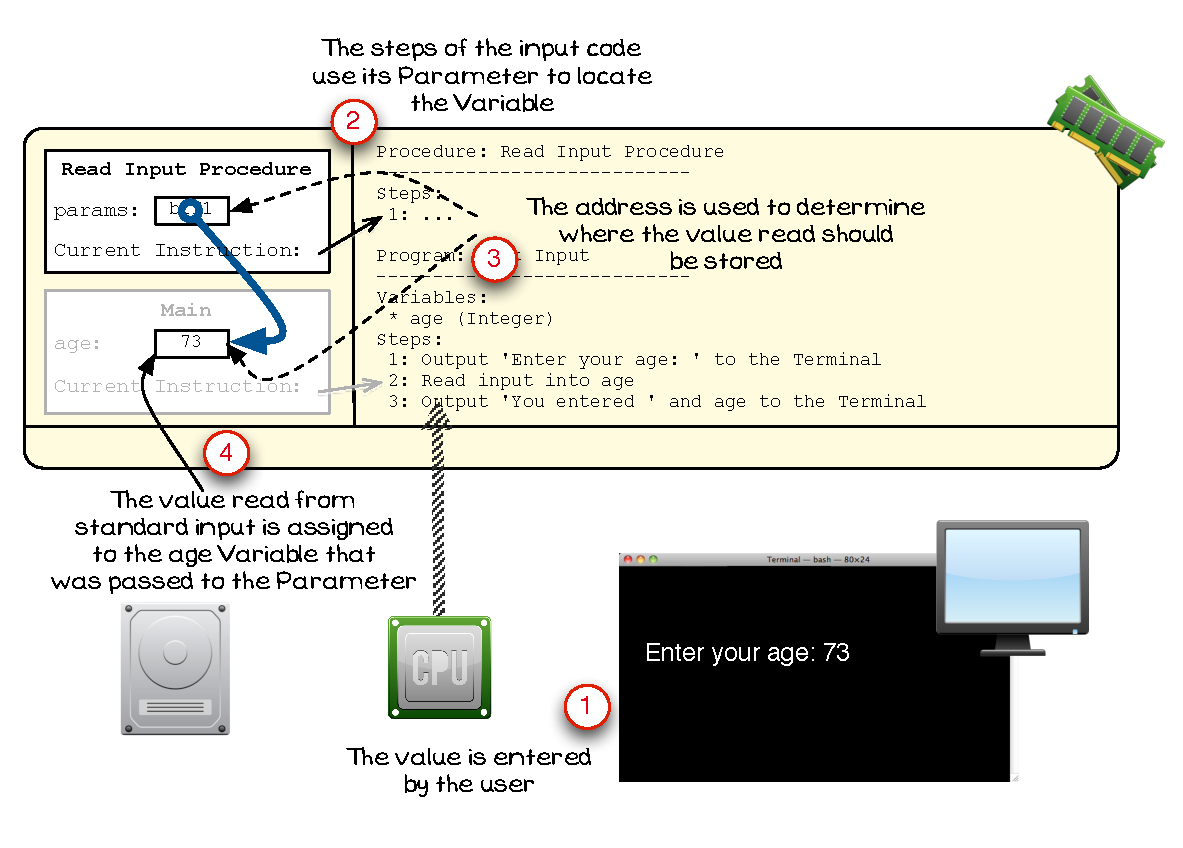
\includegraphics[width=\textwidth]{./topics/storing-using-data/images/vis-ref-3} 
   \caption{Within the input code the address is used to find where to store the value read from the user}
   \label{fig:vis-ref-3}
\end{figure}

\mynote{
\begin{itemize}
  \item In Figure \ref{fig:vis-ref-3} the indicated areas show the following:
  \begin{enumerate}
    \item The input code waits for the user to enter a value at the Terminal. Once the value is entered it is scanned and stored in the Variables passed to the Input Procedure.
    \item The input code needs to work out where the values read are to be stored. It does this by looking up the address stored in its Parameter.
    \item The address is used to locate the Variable into which the value will be stored.
    \item In this case the Parameter has the address of the \texttt{age} variable, and therefore the value read from the user is stored into Main's \texttt{age} Variable.
  \end{enumerate}
  \item The language's Input Procedures can be used to read in more than one value at a time. In these cases the inputs code will read values for each Variable one at a time.
\end{itemize}
}

\csection{In C you are responsible for determining how the data read is interpreted. This is the purpose of the \emph{format string} passed as the first parameter to \texttt{scanf}. In \csnipet{scanf("\%d", \&age);} the \texttt{"\%d"} indicates that the first Variable needs to be assigned a decimal integer value.}

% subsubsection the_input_procedure_stores_the_value_read_from_the_user_into_ (end)

\clearpage
\subsubsection{Control returns to Main and \texttt{age} has been updated with the value from the user} % (fold)
\label{ssub:control_returns_to_main_and_}

When control returns to the main code, the \texttt{age} variable has been updated to include the values read from the user.

\begin{figure}[htbp]
   \centering
   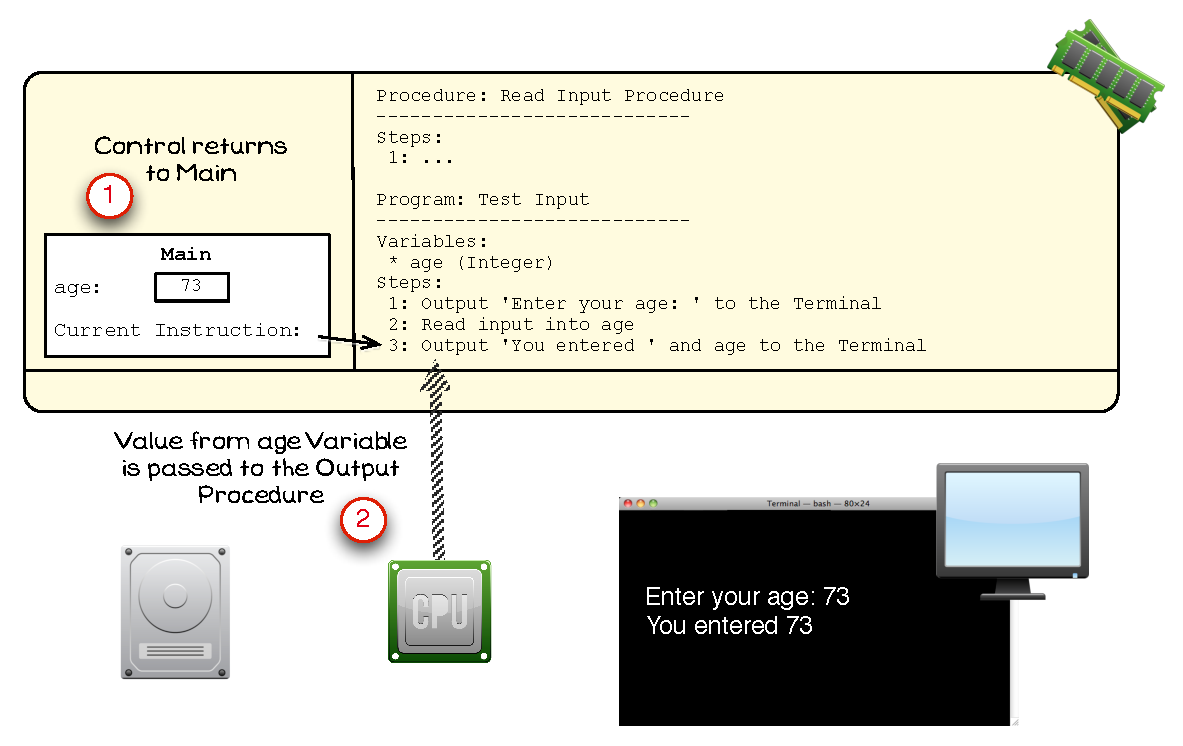
\includegraphics[width=\textwidth]{./topics/storing-using-data/images/vis-ref-4} 
   \caption{Control returns to Main, and the value of age has been updated by the input code}
   \label{fig:vis-ref-4}
\end{figure}

\mynote{
\begin{itemize}
  \item In Figure \ref{fig:vis-ref-4} the indicated areas show the following:
  \begin{enumerate}
    \item Control returns to \texttt{Main} when the input code completes.
    \item The \emph{value} from the \texttt{age} Variable is then passed to the Output procedure.
  \end{enumerate}
  \item \emph{Pass by Reference} is used when you want to pass the Variable, but in most cases you only want to pass the \emph{value} so most code uses \emph{Pass by Value}.
\end{itemize}
}

% subsubsection control_returns_to_main_and_ (end)
% subsection pass_by_reference (end)

\clearpage
\subsection{Hand Execution with Variables} % (fold)
\label{sub:hand_execution_with_variables}

One valuable skill you need to develop is the ability to step through a program in the same way the computer will. You will find that this skill will get more and more important as you progress to write larger programs. You will use this skill to help you detect and correct any \textbf{semantic errors}, in a process commonly referred to as \textbf{debugging}.

Semantic errors are errors in the logic of your program. This means that the program compiles, but does not do what you want it to. The tests that you use will help you locate these errors, but in many cases you will need to work out \emph{why} the error is occurring so that you can make the required changes.

One of the better techniques to help you make these corrections is to reading your code, and to think about the actions the computer is performing. Often these errors only require one or two lines of code to change, but before you can make these changes you need to identify \emph{where} the error is occurring, \emph{why} it is occurring, and \emph{how} you can correct the issue. By reading your code, and hand executing it you have the best chance of working out \emph{where} the problem is, and \emph{why} the problem is occurring.

These activities are very popular with Programming Tests, both in University subjects and job interviews. Being able to execute some code by hand means that you really understand what the code is doing. Once you have this level of understanding you just need to add some imagination and experience to become a very valuable software developer.

The steps you need to perform are:
\begin{itemize}
  \item \nameref{ssub:locate_the_function_or_procedure_to_test}
  \item \nameref{ssub:turn_off_your_brain}
  \item \nameref{ssub:setup_your_memory}
  \item \nameref{ssub:run_the_steps_one_at_a_time}
\end{itemize}

\subsubsection{Locate the Function or Procedure to Test} % (fold)
\label{ssub:locate_the_function_or_procedure_to_test}

Hand executing an entire program would take a very long time. As a result you want to narrow down your search to one or two Functions and/or Procedures. You can use your Structure Charts, or knowledge of the program's structure, to help you narrow down your options. Think about where the test failed, and where the code for this is located in your Program. With a small program you are likely to know immediately where the issue is, but as the program size grows it will become more difficult to know exactly where the problem is.

Listing \ref{plst:to-test} contains the pseudocode for a Procedure that will calculate and output the area of a Trapezoid. Unfortunately this code contains a number of errors. The following sections will demonstrate how to execute this procedure by hand. If this were a programming test you may be asked a question such as:
\begin{quote}
  `\emph{What is the value in area when this program is run and the user enters \textbf{5} for base 1, \textbf{7} for base 2, and \textbf{4} for height?}'
\end{quote}

Executing this by hand will give you the necessary skills to be able to answer questions such as this.

\pseudocode{plst:to-test}{Pseudocode for a Procedure that calculates the area of a Trapezoid, with errors.}{topics/storing-using-data/application/to-test.txt}

% subsubsection locate_the_function_or_procedure_to_test (end)

\subsubsection{Turn off your brain} % (fold)
\label{ssub:turn_off_your_brain}

Once you have located the Function or Procedure that you need to test you can start to execute it. The main obstacle in most peoples way is, unfortunately, their brain. You are going to \emph{think} about what you \emph{wanted} the program to do. This is something the computer \emph{cannot} do. The computer is unintelligent. It is a machine that does as you command. To run this program as the computer does you will need to \textbf{stop thinking} and start doing as commanded.

Rules:
\begin{itemize}
  \item Do not think about what you \emph{want} or \emph{expect} the program to do.
  \item Perform the commands as they are, one at a time
  \item You cannot remember anything that is not written down.
  \item Focus only on the current command (Statement). Do not look at other Statements!
  \item Perform the actions you are commanded to perform, and only those actions. Do not do more than you are commanded to.
  \item Use the language's Statements to determine the actions you must perform:
  \begin{itemize}
    \item An \nameref{sub:assignment_statement} will evaluate its expression, and assign a value to a variable.
    \item A \nameref{sub:procedure call} runs the code in a Procedure, a \nameref{sub:function_call} runs the code in a Function. To optimise this step you can perform the actions within called Functions or Procedures without stepping through their code in most cases.
  \end{itemize}
\end{itemize}

% subsubsection turn_off_your_brain (end)

\clearpage
\subsubsection{Setup your `memory'} % (fold)
\label{ssub:setup_your_memory}

One of the rules when running your code by hand is that you can not remember anything. The values you use must come from the `memory' that you setup for the Function or Procedure. So, the first step for executing this code performs the actions that called the procedure: you need to \emph{allocate space} on the stack. You can simulate this using a piece of paper. This piece of paper will be the `memory' used by the code as it executes. To set this memory up you will need to do the following:

\begin{enumerate}
  \item Get a blank piece of paper.
  \item Write \texttt{Print Trapezoid Area} to remember that is the procedure you are in.
  \item Do the following for any Variables\footnote{Draw boxes for Parameters, Local Variables, and Function results.} in the Function or Procedure:
  \begin{enumerate}
    \item \textbf{Draw a box} to represent the Variable. Make sure that it is large enough for you to write values inside.
    \item \textbf{Write the name} of the Variable next to the box.
    \item If the Variable is a Parameter, copy the value from the argument into the box, otherwise leave it empty.
  \end{enumerate}
\end{enumerate}

When you have finished these steps for the code in Listing \ref{plst:to-test} you should have a piece of paper that looks like the image in Figure \ref{fig:hand-exe-1}. The empty boxes represent the different Variables, the fact we have not written a Value into these boxes tells us that at this point the value has not been set, and therefore should not be used.

\begin{figure}[htbp]
   \centering
   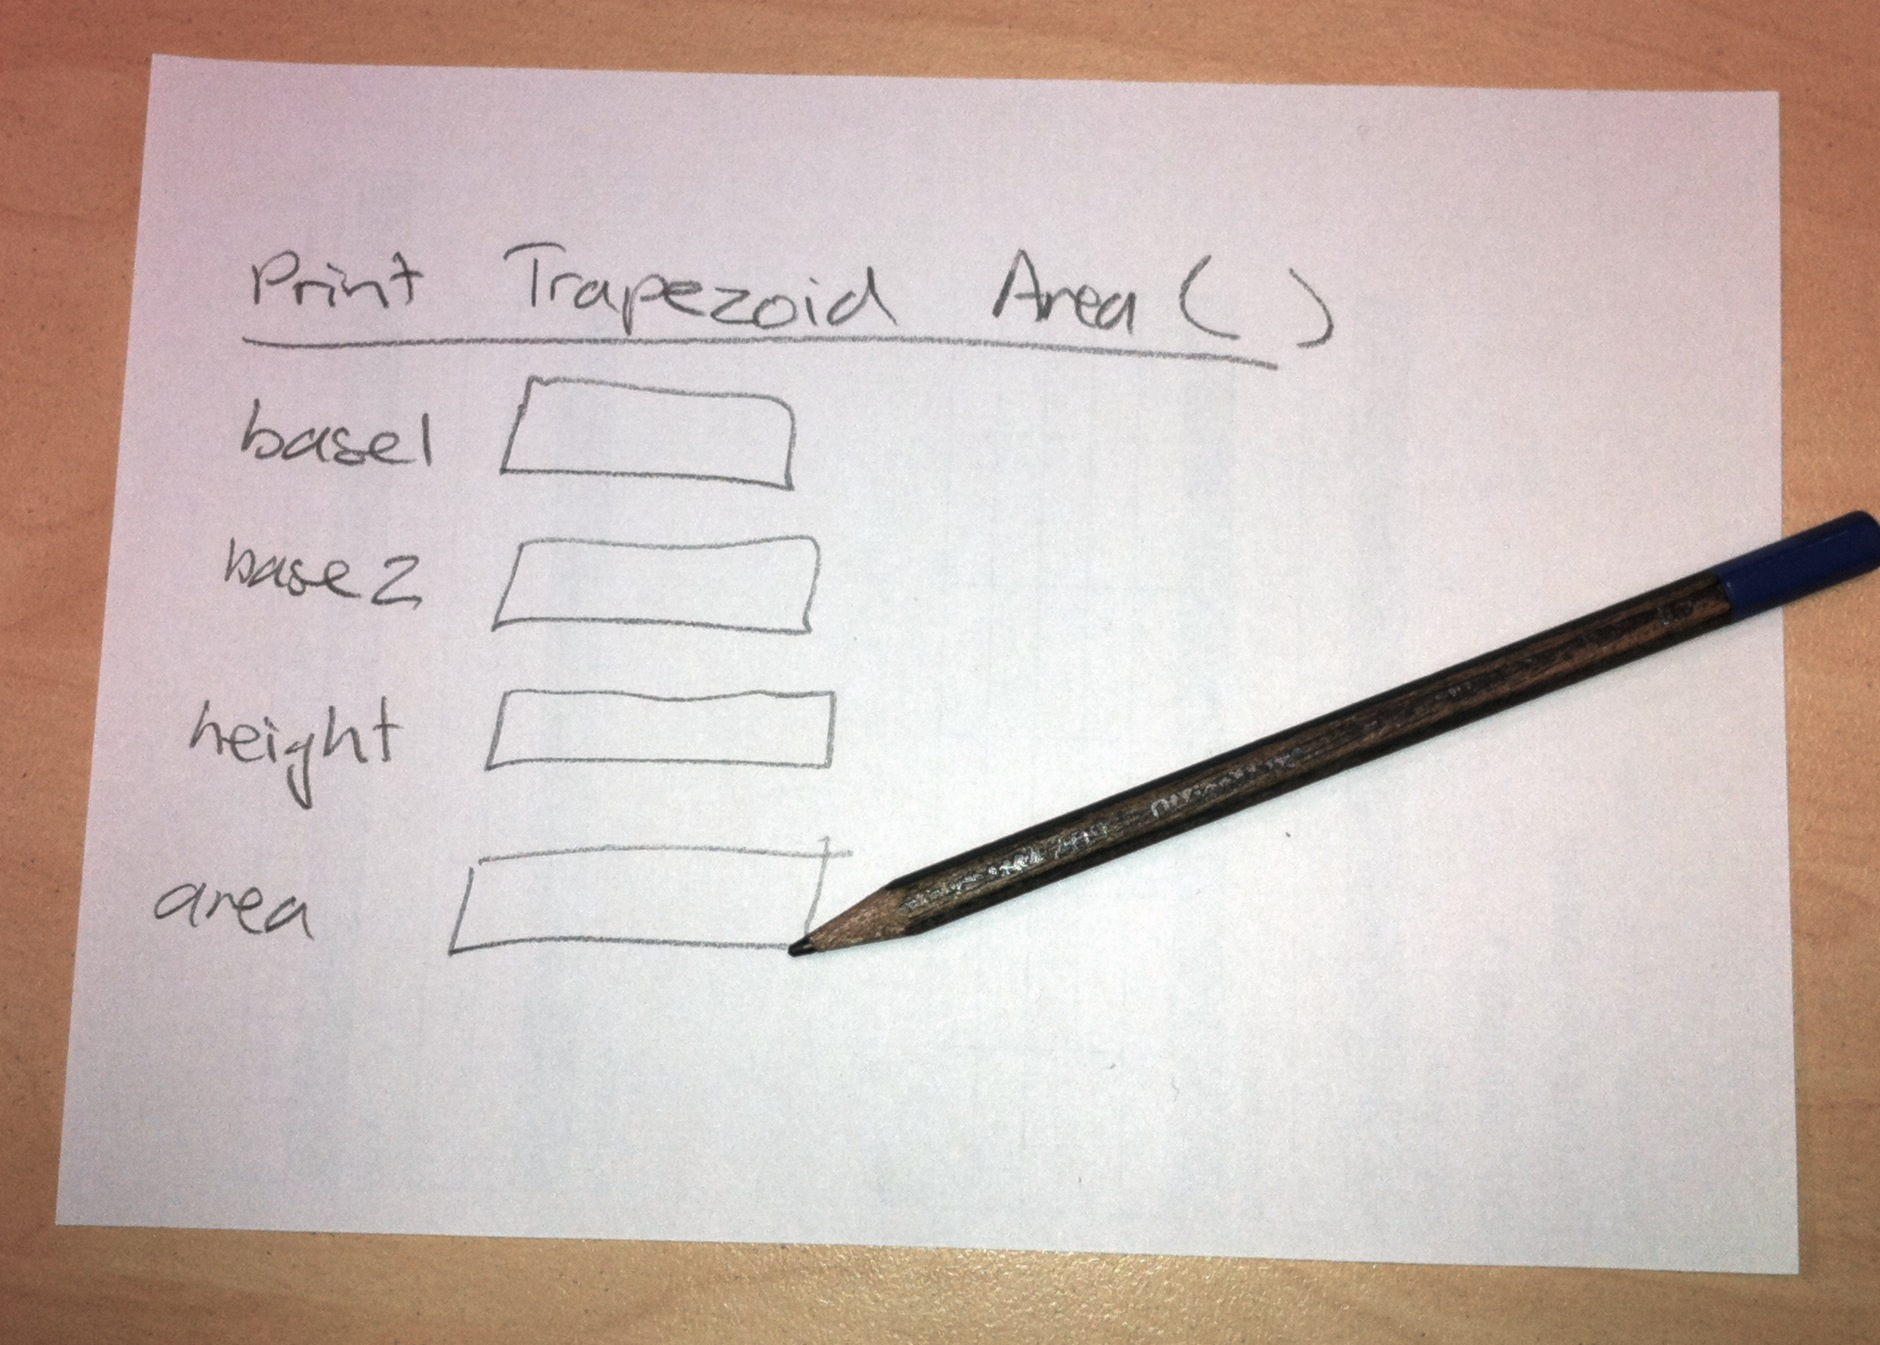
\includegraphics[width=0.7\textwidth]{./topics/storing-using-data/images/hand-exe-1} 
   \caption{Draw space for all of the Function or Procedure's Variables}
   \label{fig:hand-exe-1}
\end{figure}

% subsubsection setup_your_memory (end)

\clearpage
\subsubsection{Run the steps one at a time} % (fold)
\label{ssub:run_the_steps_one_at_a_time}

Now that the memory has been initialised it is time to run each instruction in the code. You need to do this \textbf{one instruction at a time}. It does not matter how large the code is, the computer will always run it one Statement at a time. Do not think, just read the Statement and perform the action.

\begin{enumerate}
  \item Step 1 calls the output procedure of the Language. This will output the text `\emph{Enter base 1: }' to the Terminal. You do not need to step into the internal actions of each Function or Procedure called, as long as you can replicate the actions that it would perform. If you had been asked `\emph{What is output by the the call to \texttt{Print Trapezoid Area}?}' it would be important to put this in the answer, but as we just want to know the final result you can skip this.
  \item Step 2 reads a value from the user and stores it in \texttt{base1}. The user is responding to the prompt from step 1, and therefore enters \emph{5}, the value indicated in the question. As the \texttt{base1} variable is passed to this call you now write \textbf{5} into the \texttt{base1} box, representing the fact that this Variable now has the value \emph{5}. See Figure \ref{fig:hand-exe-2}.
  \item Step 3 outputs the next prompt, `\emph{Enter base 2: }'.
  \item Step 4 reads a value from the user, and stores it in \textbf{\texttt{base1}}. This is the source of the first error. This is most likely the result of a copy/paste error, where the developer has copied the instructions to prompt the user and read a value into \texttt{base1}, and then changed it to read a value into \texttt{base2}. When you copy and paste code you need to pay extra attention to making sure that the pasted code is changed correctly.\newline\newline When this code is run a new value will be written into the \texttt{base1} Variable. Cross out the old value, and write in the new value. The value entered in this case is \textbf{7}, as indicated in the question. See Figure \ref{fig:hand-exe-3}.
  \item Step 5 outputs the prompt for height.
  \item Step 6 reads \textbf{4} from the user and stores it into the \texttt{height} Variable. See Figure \ref{fig:hand-exe-4}
  \item Step 7 now reads the values from \texttt{height}, and \texttt{base1}. The equation for calculating the area of a Trapezoid is $ height ( \frac{base 1 + base 2}{2} ) $, this has been coded incorrectly again, with several errors. Firstly \texttt{base1} is read twice, and \texttt{base2} is not used at all. Second, using BODMAS the current code is actually performing the equation $ height (base 1 + \frac{base 1}{2})$. Performing this calculation you will find that the value stored in \texttt{area} is $ 4 ( 7 + (7 / 2)) = 42$.
  \item Step 8 outputs the area to the Terminal, displaying `\emph{Trapezoid area is 42}'. See Figure \ref{fig:hand-exe-5}.
\end{enumerate} 

At this point the Procedure has ended, and you have collected all of the details about how the program actually works. You need to use this information to determine where the error is. If this failed to find the problem then the problem may be located elsewhere in the Program's code, or you have misread something. Getting someone else to help you debug your programs is always a good option, they are likely to see things that you may miss as the code's developer.

\mynote{
\begin{itemize}
  \item Pay careful attention to exactly what the statement is getting the computer to do.
  \item Proceed slowly and carefully, as mistakes can be as small as a single character in the wrong place.
  \item Make sure that you are aware of exactly what the different Statements do, and how they work.
  \item Always use the values of the Variables from `\emph{memory}', i.e. read/write them on to your piece of paper. 
\end{itemize}
}

\begin{figure}[htbp]
   \centering
   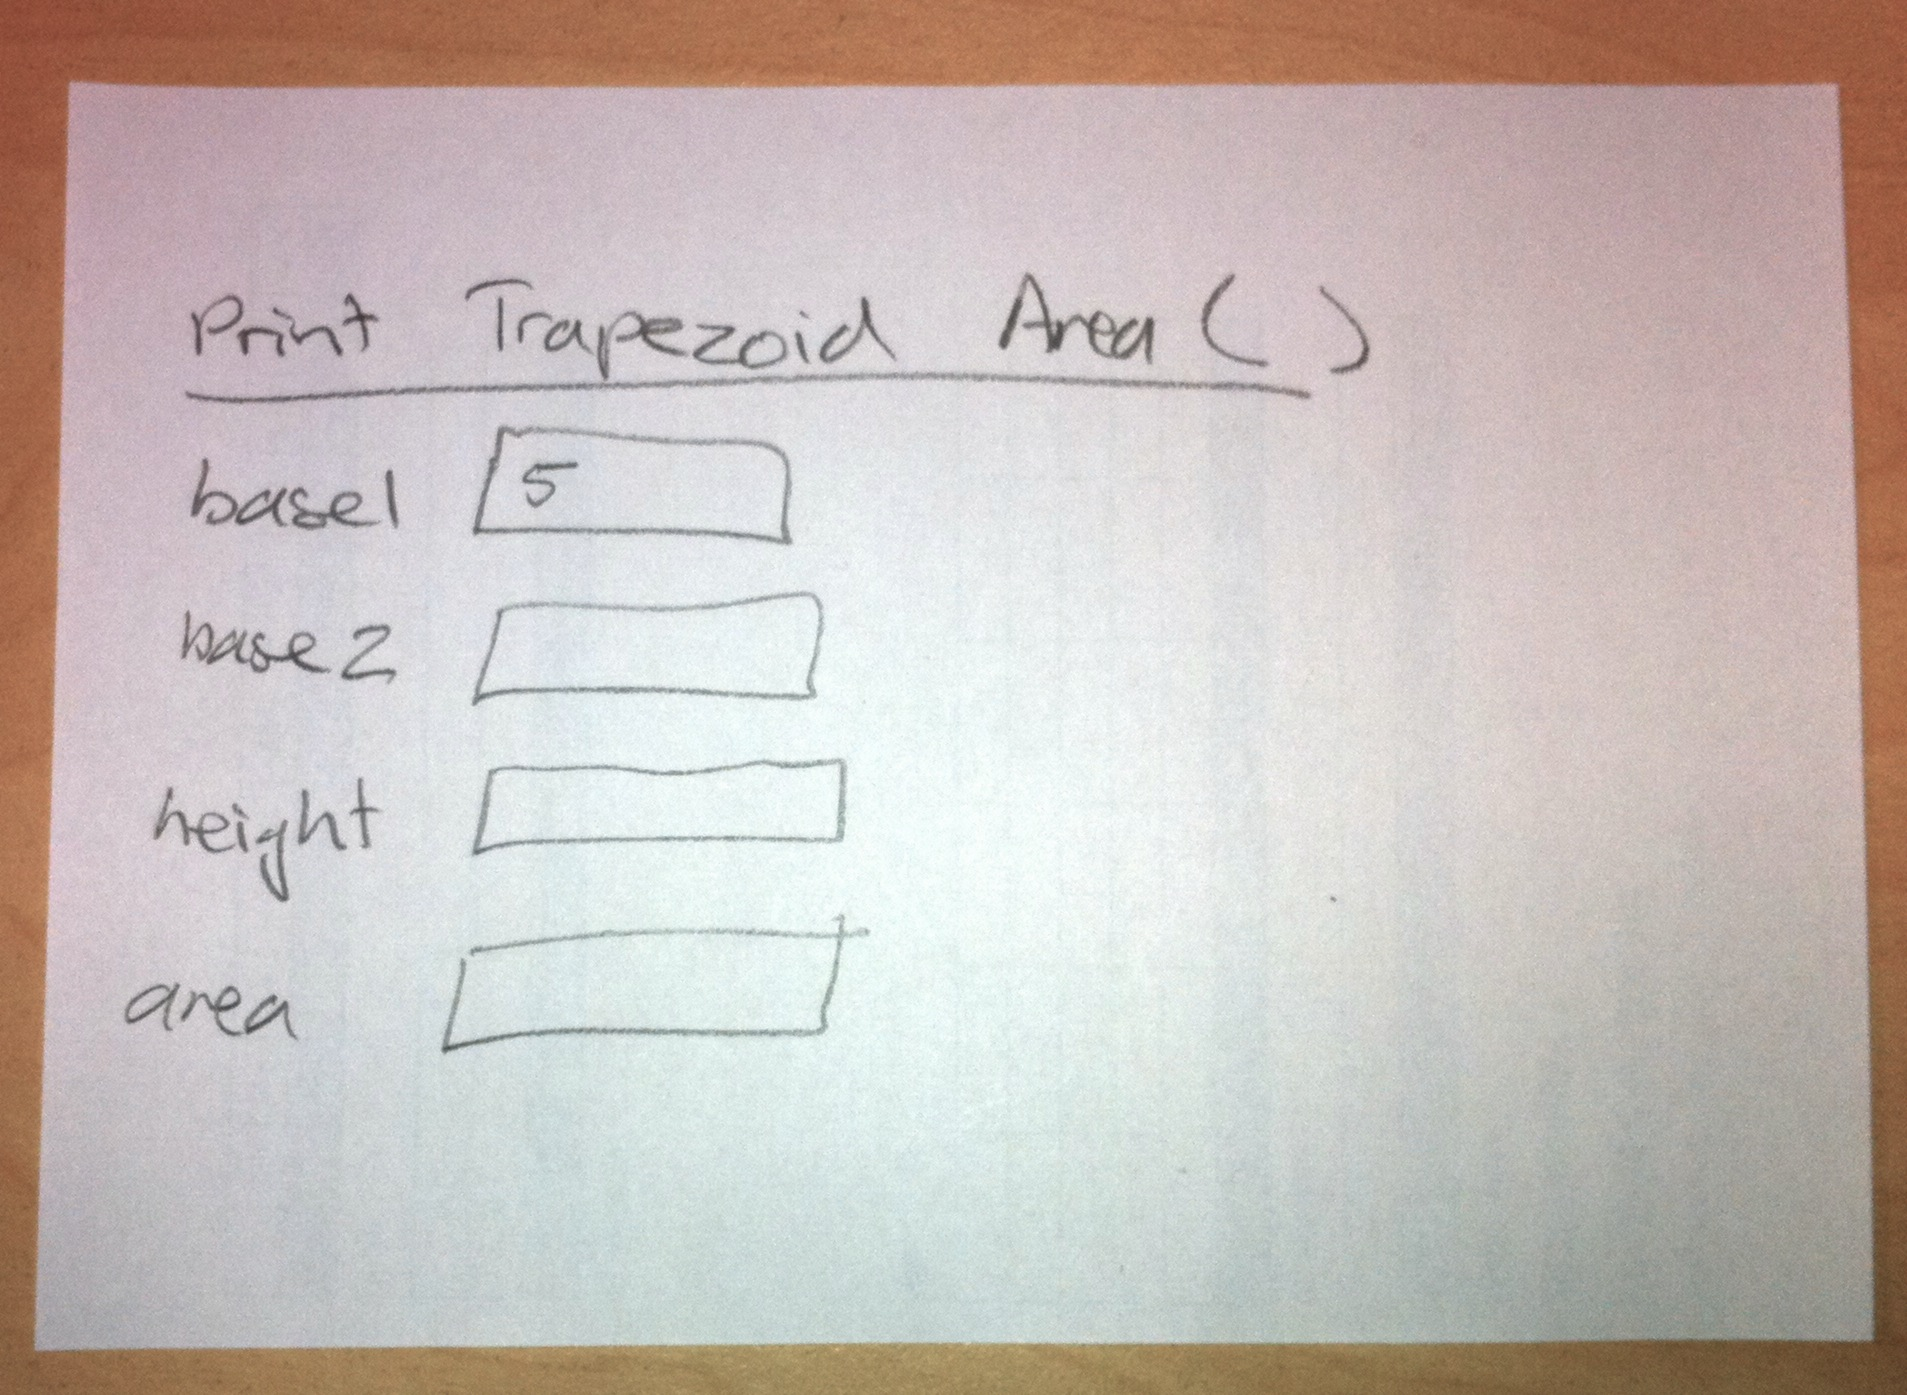
\includegraphics[width=0.7\textwidth]{./topics/storing-using-data/images/hand-exe-2} 
   \caption{The value 5 is stored in the \texttt{base1} Variable}
   \label{fig:hand-exe-2}
\end{figure}

\begin{figure}[htbp]
   \centering
   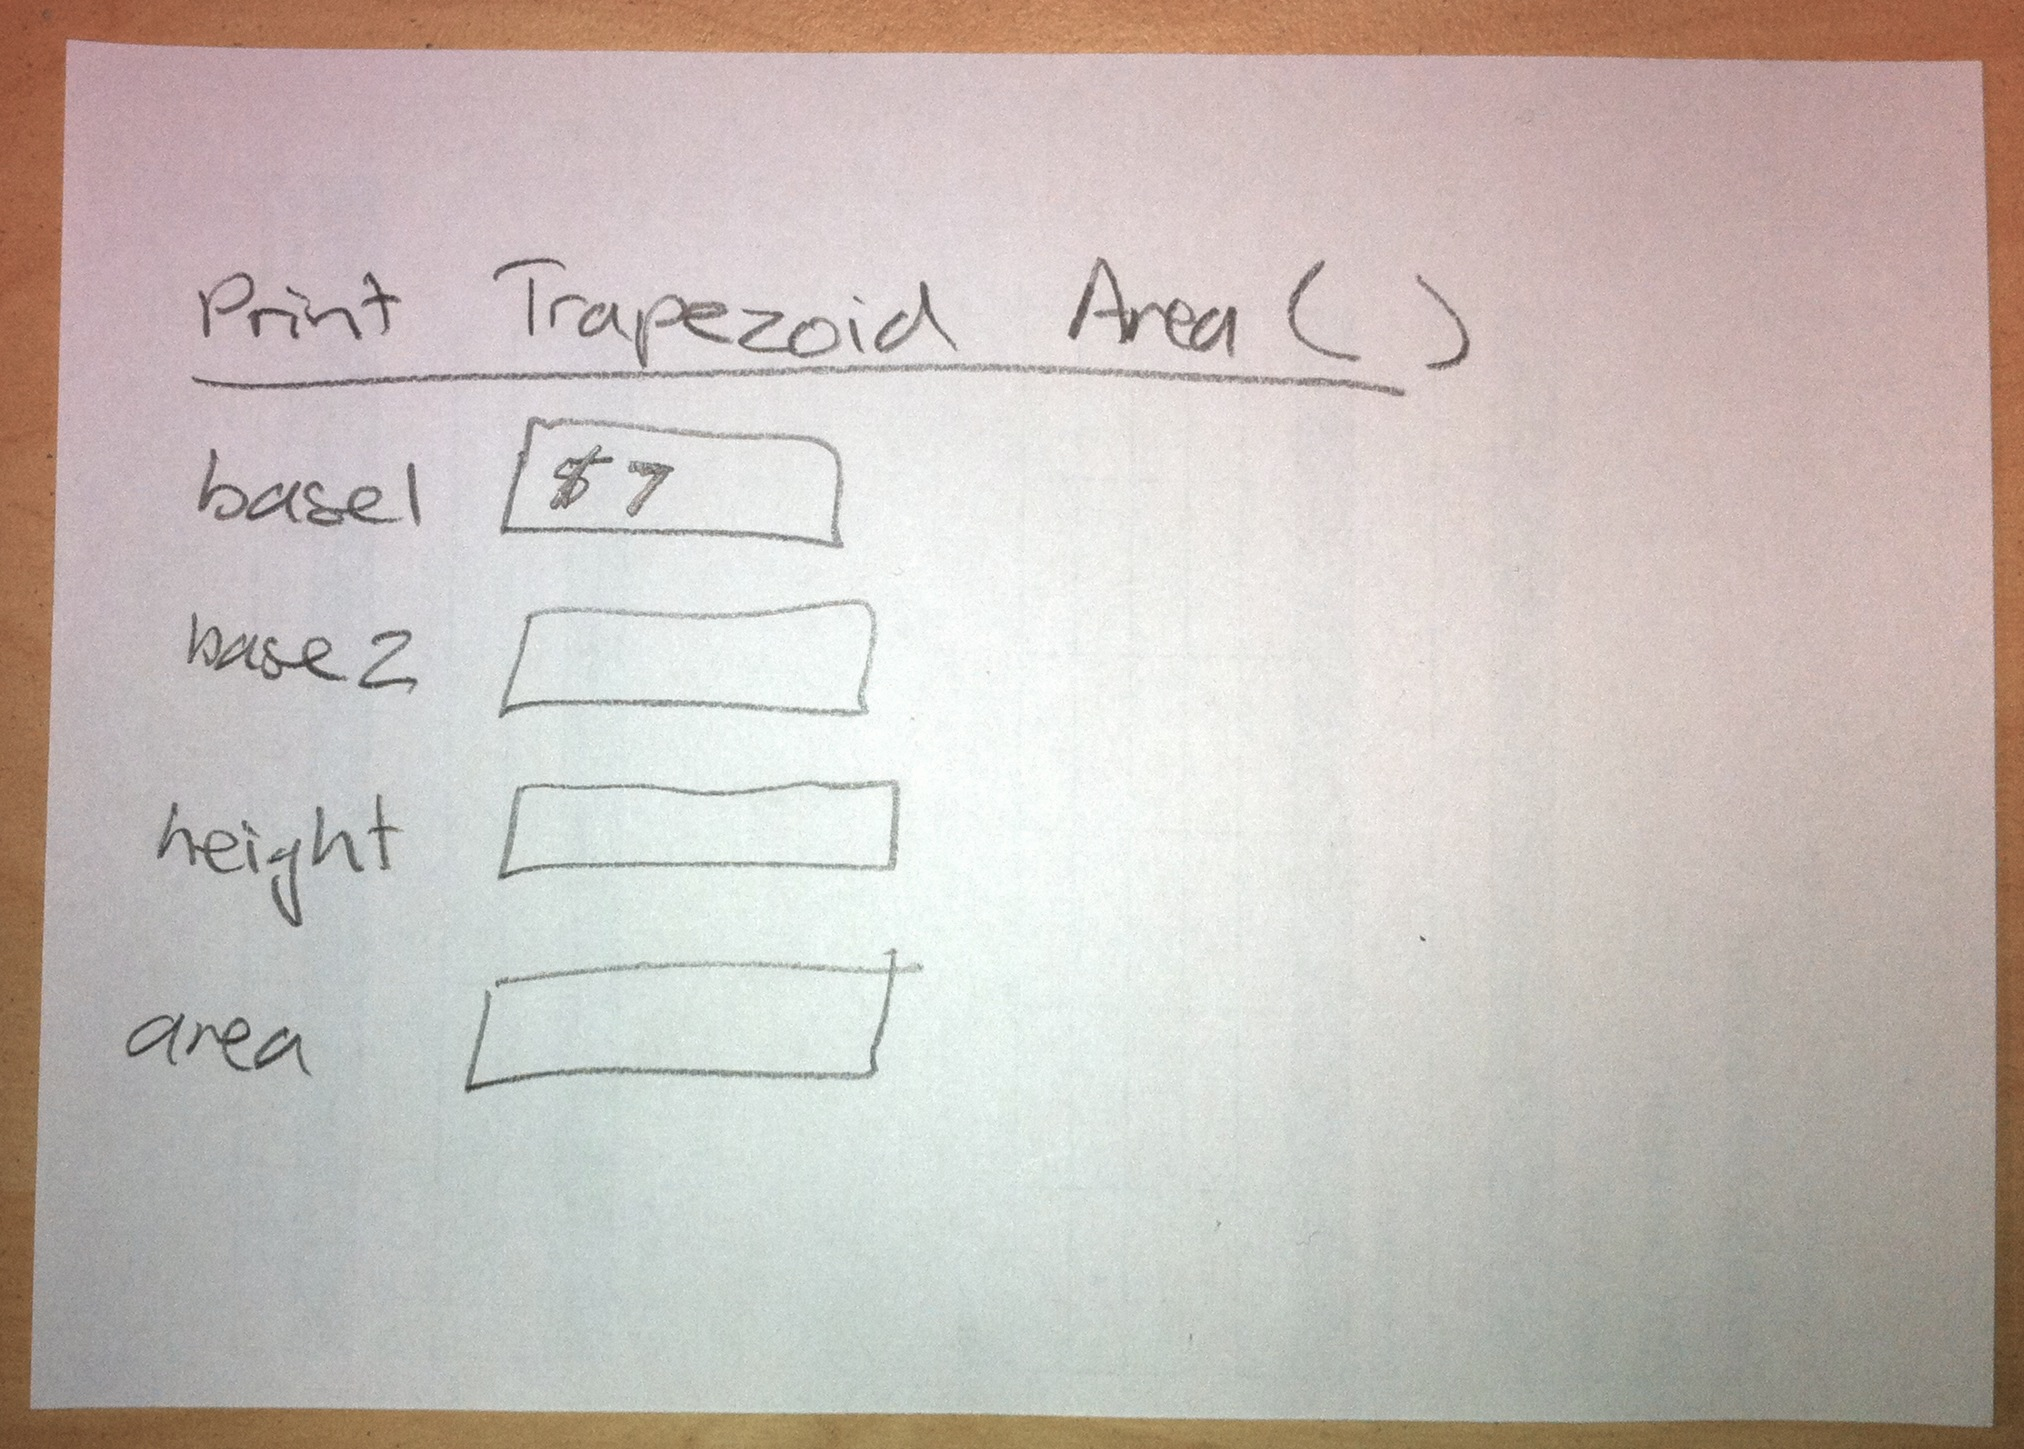
\includegraphics[width=0.7\textwidth]{./topics/storing-using-data/images/hand-exe-3} 
   \caption{The value 7 is stored in the \texttt{base1} Variable}
   \label{fig:hand-exe-3}
\end{figure}

\begin{figure}[htbp]
   \centering
   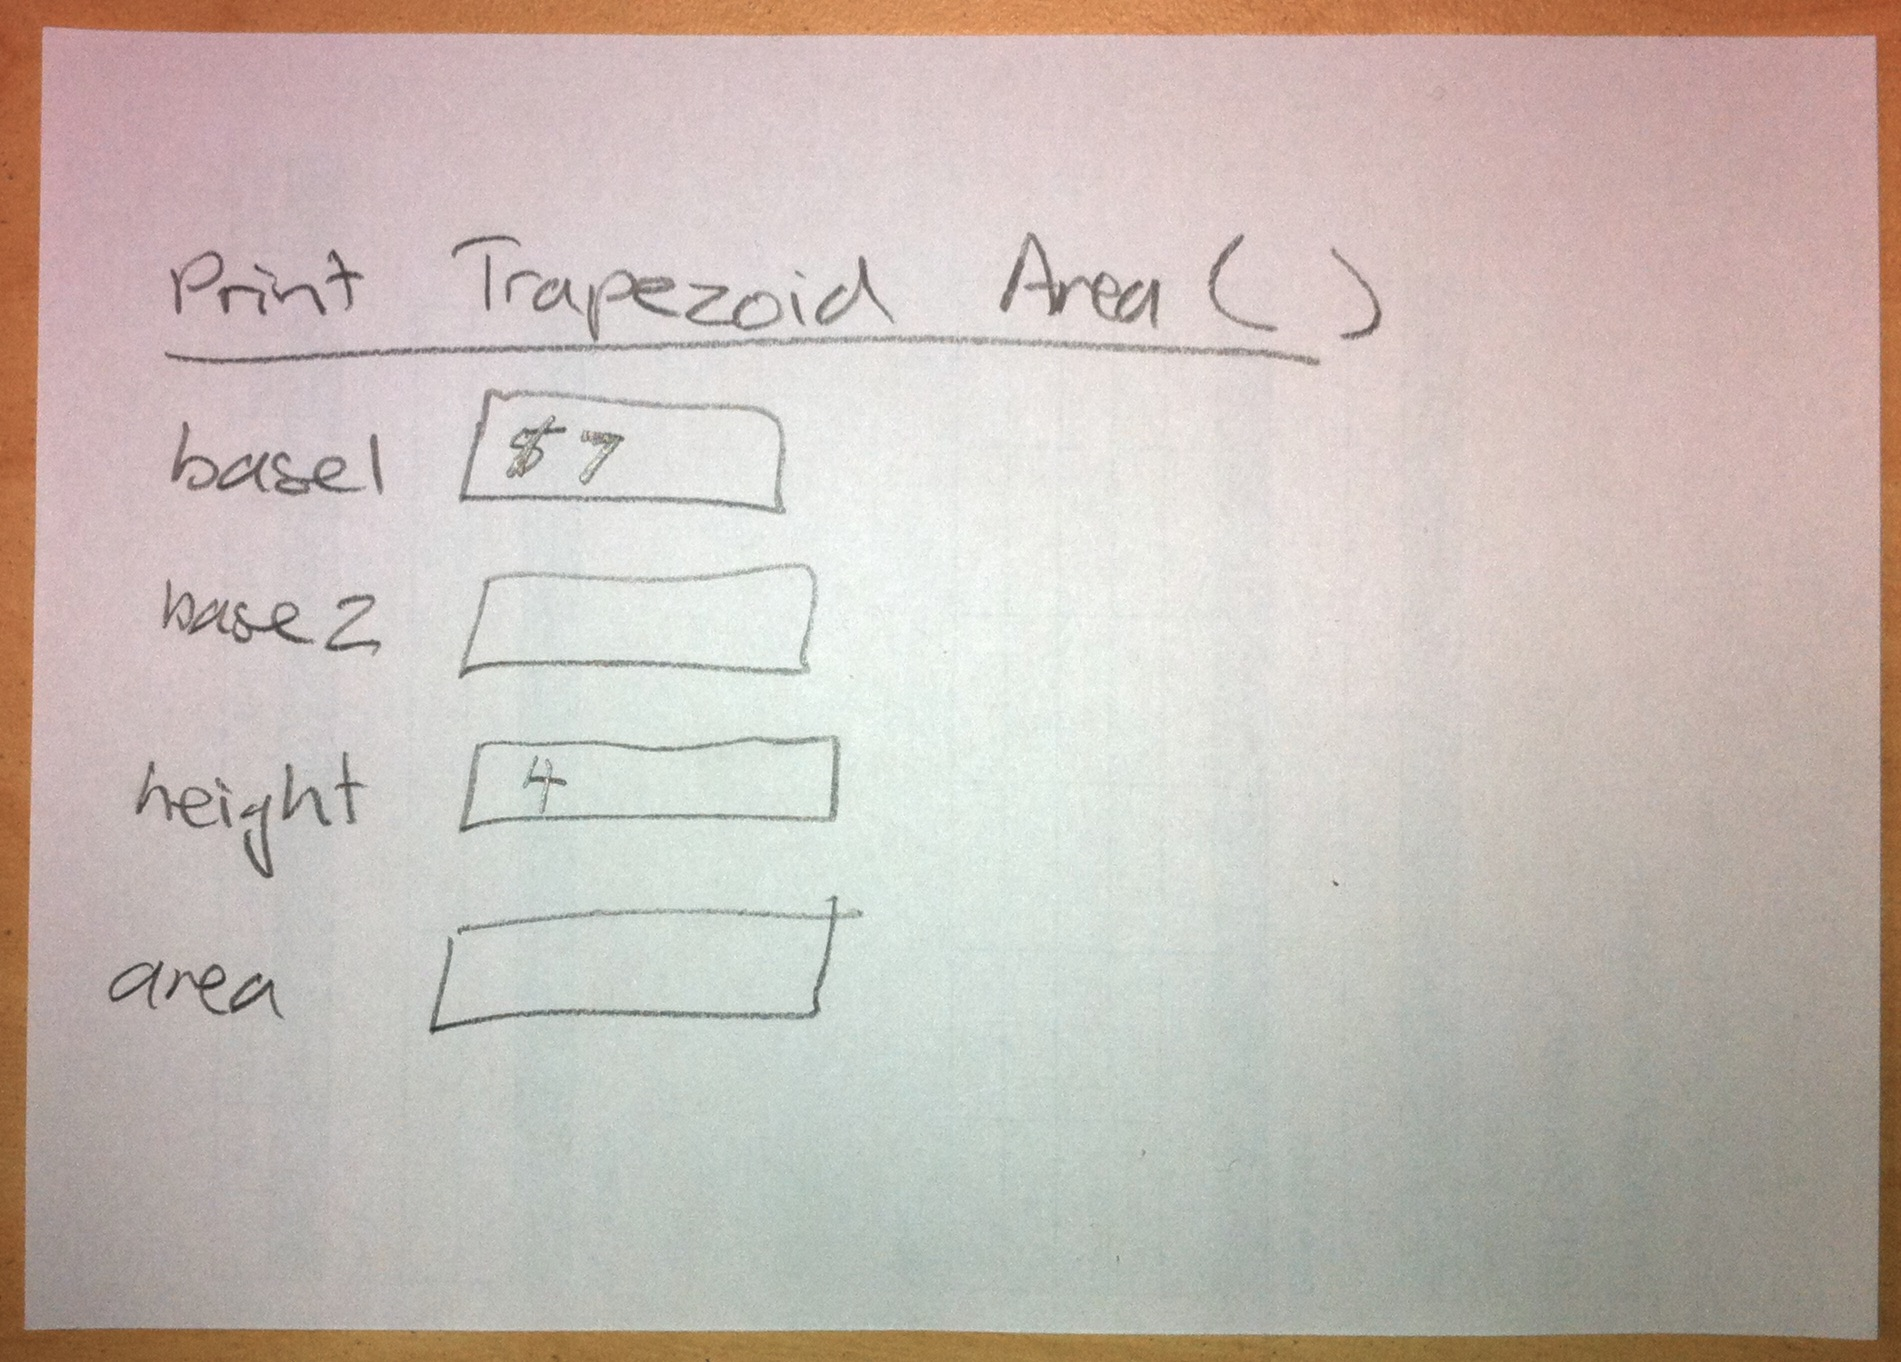
\includegraphics[width=0.7\textwidth]{./topics/storing-using-data/images/hand-exe-4} 
   \caption{The value 4 has been stored in \texttt{height}}
   \label{fig:hand-exe-4}
\end{figure}

\begin{figure}[htbp]
   \centering
   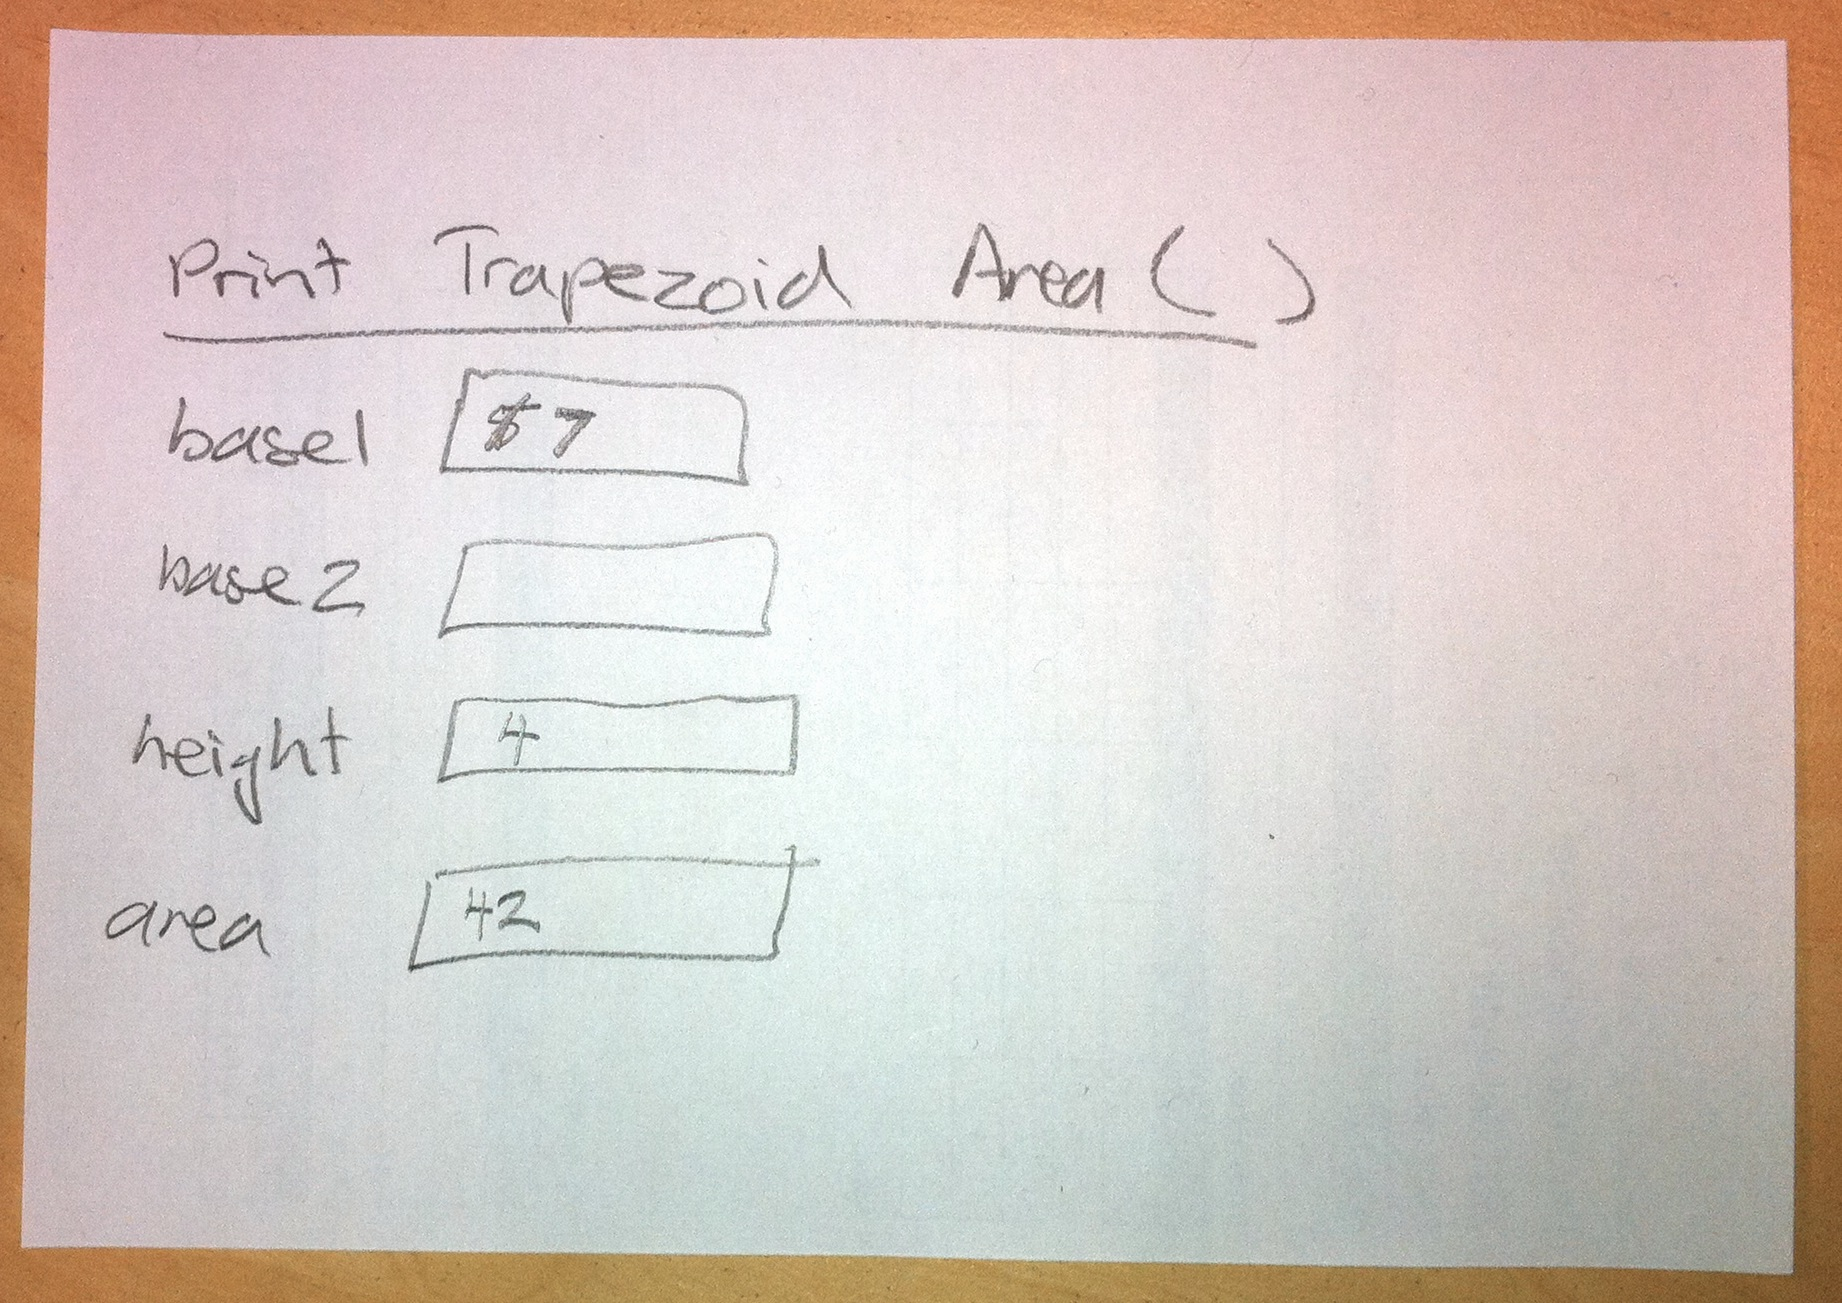
\includegraphics[width=0.7\textwidth]{./topics/storing-using-data/images/hand-exe-5} 
   \caption{The value 42 is stored in \texttt{area}}
   \label{fig:hand-exe-5}
\end{figure}

% subsubsection run_the_steps_one_at_a_time (end)
% subsection hand_execution_with_variables (end)

\clearpage
\subsection{Summary} % (fold)
\label{sub:visualise_data_summary}

In this Section you have seen how Variables work within the Computer, and been introduced to the idea of Functions. With these concepts you can now work more meaningfully with the data in your programs.

\bigskip
\mynote{
\begin{itemize}
  \item A Variable has two main aspects:
  \begin{itemize}
    \item The \textbf{Variable} itself, a space in memory. You can think of this like a box, into which a value can be placed.
    \item The \textbf{value} that is stored within the Variable.
  \end{itemize}
  \item Variables can be declared in one of three locations:
  \begin{itemize}
    \item \textbf{Local Variables} are declared within Functions and Procedures.
    \item \textbf{Parameters} are also declared within Functions and Procedures, but are given a value as part of the call to this code.
    \item \textbf{Global Variables} are declared within the Program, and are accessible within all Functions and Procedures.
  \end{itemize}
  \item The \textbf{Assignment Statement} can be used to store a value in a Variable. The \emph{left hand side} of an assignment is a Variable, the \emph{right hand side} is an Expression.
  \item You can read the \emph{value} of a Variable in an \textbf{Expression}.
  \item When you call a Function or a Procedure you can pass the Parameter either \textbf{by value} or \textbf{by reference}. When passed \emph{by reference} the Parameter must be passed a Variable.
  \item A \textbf{Function} is just like a Procedure, except that it returns a result and is therefore called inside Expressions so that the returned value can be used.
  \item A \textbf{Function} is called to \emph{calculate a value}.
\end{itemize}
}

% subsection summary (end)